\documentclass[twoside]{book}

% Packages required by doxygen
\usepackage{fixltx2e}
\usepackage{calc}
\usepackage{doxygen}
\usepackage[export]{adjustbox} % also loads graphicx
\usepackage{graphicx}
\usepackage[utf8]{inputenc}
\usepackage{makeidx}
\usepackage{multicol}
\usepackage{multirow}
\PassOptionsToPackage{warn}{textcomp}
\usepackage{textcomp}
\usepackage[nointegrals]{wasysym}
\usepackage[table]{xcolor}

% Font selection
\usepackage[T1]{fontenc}
\usepackage[scaled=.90]{helvet}
\usepackage{courier}
\usepackage{amssymb}
\usepackage{sectsty}
\renewcommand{\familydefault}{\sfdefault}
\allsectionsfont{%
  \fontseries{bc}\selectfont%
  \color{darkgray}%
}
\renewcommand{\DoxyLabelFont}{%
  \fontseries{bc}\selectfont%
  \color{darkgray}%
}
\newcommand{\+}{\discretionary{\mbox{\scriptsize$\hookleftarrow$}}{}{}}

% Page & text layout
\usepackage{geometry}
\geometry{%
  a4paper,%
  top=2.5cm,%
  bottom=2.5cm,%
  left=2.5cm,%
  right=2.5cm%
}
\tolerance=750
\hfuzz=15pt
\hbadness=750
\setlength{\emergencystretch}{15pt}
\setlength{\parindent}{0cm}
\setlength{\parskip}{3ex plus 2ex minus 2ex}
\makeatletter
\renewcommand{\paragraph}{%
  \@startsection{paragraph}{4}{0ex}{-1.0ex}{1.0ex}{%
    \normalfont\normalsize\bfseries\SS@parafont%
  }%
}
\renewcommand{\subparagraph}{%
  \@startsection{subparagraph}{5}{0ex}{-1.0ex}{1.0ex}{%
    \normalfont\normalsize\bfseries\SS@subparafont%
  }%
}
\makeatother

% Headers & footers
\usepackage{fancyhdr}
\pagestyle{fancyplain}
\fancyhead[LE]{\fancyplain{}{\bfseries\thepage}}
\fancyhead[CE]{\fancyplain{}{}}
\fancyhead[RE]{\fancyplain{}{\bfseries\leftmark}}
\fancyhead[LO]{\fancyplain{}{\bfseries\rightmark}}
\fancyhead[CO]{\fancyplain{}{}}
\fancyhead[RO]{\fancyplain{}{\bfseries\thepage}}
\fancyfoot[LE]{\fancyplain{}{}}
\fancyfoot[CE]{\fancyplain{}{}}
\fancyfoot[RE]{\fancyplain{}{\bfseries\scriptsize Generated by Doxygen }}
\fancyfoot[LO]{\fancyplain{}{\bfseries\scriptsize Generated by Doxygen }}
\fancyfoot[CO]{\fancyplain{}{}}
\fancyfoot[RO]{\fancyplain{}{}}
\renewcommand{\footrulewidth}{0.4pt}
\renewcommand{\chaptermark}[1]{%
  \markboth{#1}{}%
}
\renewcommand{\sectionmark}[1]{%
  \markright{\thesection\ #1}%
}

% Indices & bibliography
\usepackage{natbib}
\usepackage[titles]{tocloft}
\setcounter{tocdepth}{3}
\setcounter{secnumdepth}{5}
\makeindex

% Hyperlinks (required, but should be loaded last)
\usepackage{ifpdf}
\ifpdf
  \usepackage[pdftex,pagebackref=true]{hyperref}
\else
  \usepackage[ps2pdf,pagebackref=true]{hyperref}
\fi
\hypersetup{%
  colorlinks=true,%
  linkcolor=blue,%
  citecolor=blue,%
  unicode%
}

% Custom commands
\newcommand{\clearemptydoublepage}{%
  \newpage{\pagestyle{empty}\cleardoublepage}%
}

\usepackage{caption}
\captionsetup{labelsep=space,justification=centering,font={bf},singlelinecheck=off,skip=4pt,position=top}

%===== C O N T E N T S =====

\begin{document}

% Titlepage & ToC
\hypersetup{pageanchor=false,
             bookmarksnumbered=true,
             pdfencoding=unicode
            }
\pagenumbering{alph}
\begin{titlepage}
\vspace*{7cm}
\begin{center}%
{\Large M\+T\+Unit Help \\[1ex]\large v1.\+0 }\\
\vspace*{1cm}
{\large Generated by Doxygen 1.8.14}\\
\end{center}
\end{titlepage}
\clearemptydoublepage
\pagenumbering{roman}
\tableofcontents
\clearemptydoublepage
\pagenumbering{arabic}
\hypersetup{pageanchor=true}

%--- Begin generated contents ---
\chapter{R\+E\+A\+D\+ME}
\label{index}\hypertarget{index}{}\section*{\mbox{\hyperlink{class_m_t_unit}{M\+T\+Unit}} -\/ A Unit Test framework for Meta\+Trader 5}

This project consists in a powerful Unit Test Framework for Meta\+Trader 5.

It was originally based on this article\+: \href{https:/www.mql5.com/ru/articles/1579}{\tt https\+:/www.\+mql5.\+com/ru/articles/1579}

As you might know, Meta\+Trader does not provide any kind of tool for unit testing natively. And that is probably the reason you are here.

My goal here was to develop a tool to help me applying Test-\/\+Driven-\/\+Development in my Expert Advisors. A wise decision since my E\+As will be dealing with MY P\+R\+E\+C\+I\+O\+US M\+O\+N\+E\+Y!

This project is a set of many tools that work together so that the whole process can be automated. Let me summarize some features, then.

\subsubsection*{First of all\+: The Unit Test}

It contains basically all the common assert methods used in unit testing.

If you need something more specific, you just need to implement yourself following the examples. The \mbox{\hyperlink{class_m_t_unit}{M\+T\+Unit}} executes all the existing test cases of all test suites present in the Test folder. It reports time spent, number of asserts and tests executed, and also messages whether a test passes or fails (really?).

The Unit Test itself is amazing but since it is not integrated with Meta\+Editor, it needs some manual procedures in order to work. For example, for each test written, the following workflow should be used to obtain more complete output results\+: test\+Case\+Init(), set\+Up(), test\+Case(), tear\+Down(), test\+Case\+De\+Init().

Also, the Test\+Suite should be init and de\+Init once, and the Unit Test library need to be aware of which testing suites it should execute, being necessary to instantiate an object of each test\+Suite somewhere in the Unit Test.

Yes, you can just copy and paste and change the test names, so it\textquotesingle{}s not a big deal after everything is set up...

But this is a lot of manual work and it is enough for many people quit unit testing.

There comes the second tool...

\subsubsection*{2º Tool\+: M\+T\+Unit\+Tests\+Compiler}

This tool goes through all files in the Test folder and generates an output file (\mbox{\hyperlink{_m_t_unit_all_tests_8mqh}{M\+T\+Unit\+All\+Tests.\+mqh}}) containing all declarations and initializations for all tests. This unique file is used by the Unit Test and you don\textquotesingle{}t even need to touch it. The only thing you need to do is write your tests inside the Test folder.

But... Isn\textquotesingle{}t it frustrating to have to execute this tool every time I write or modify a new test??? If you are questioning yourself about this, welcome to the club of the lazy ones! (Nice to meet you, I\textquotesingle{}m the president!).

Guess what? I\textquotesingle{}ve made two solutions for you...

The first one is the simplest one and probably will be all you need (or not, if you are ok in writing the setups for your tests manually).


\begin{DoxyItemize}
\item There is a Watcher mode that monitors any change inside the Test directory. To enter this mode, just double click the file mt\+Unit\+Helper.\+exe inside the Runners folder.
\end{DoxyItemize}

\begin{DoxyNote}{Note}
Important\+: If you are cool in using Meta\+Editor, it\textquotesingle{}s fine, you are done here. But if you are not so happy with Meta\+Editor limitations, I suggest you to continue this reading.
\end{DoxyNote}
The second solution is more intense... Let\textquotesingle{}s talk about environment.


\begin{DoxyCode}
The environment should be protected at any cost! Stop polluting and please recycle your trash!
\end{DoxyCode}
 No no no, not this kind of environment... Here is the thing, I particularly do not like to use the Meta\+Editor, it seems to be very limited in some important aspects.

So, the solution was to set up Sublime Text 3 (\href{http:/www.sublimetext.com}{\tt http\+:/www.\+sublimetext.\+com}) to open .mq5 and .mqh files, apply syntax highlight, build, run the tests and show the output. In order to do that, some scripts are used in Sublime.

The first one is\+: sublime\+\_\+mql5 (a very suggestive name, indeed)

The original version can be found on\+: \href{https:/github.com/rodrigopandini/sublime_mql5}{\tt https\+:/github.\+com/rodrigopandini/sublime\+\_\+mql5}

I\textquotesingle{}ve made some modifications because the feature \char`\"{}\+Go to definition\char`\"{} was not working as well as a few other minor issues. The version I\textquotesingle{}m using right know is included inside the \char`\"{}\+Other\char`\"{} folder. This plugin executes a .bat file during the build phase, this .bat file is responsible for executing the M\+T\+Unit\+Tests\+Compiler tool,as well as the following (and last) two tools I am going to explain next.

In order to run the tests, it is necessary to execute the Meta\+Terminal. Meta\+Terminal needs to know the simulation parameters we want to use and to do so, it asks for a config file containing such parameters. One of these parameters is the \char`\"{}\+Expert\char`\"{}, which is the path to the Expert Advisor we are testing. In order to update this Expert param, this config file should be updated with whatever Expert you are willing to test... And you don\textquotesingle{}t want to bother in doing something like that, do you?

\subsubsection*{3º Tool\+: M\+T\+Unit\+E\+A\+Linker}

So I present you the M\+T\+Unit\+E\+A\+Linker (good name, right? I\textquotesingle{}m very creative, I know that).

The only thing it does is update that param. Yes, simple as pie, but it was needed. The configuration file used is called auto\+Run\+Test.\+ini. \begin{DoxyNote}{Note}
You don\textquotesingle{}t need to interact with this tool. It\textquotesingle{}s called automatically in the build script on Sublime Text.
\end{DoxyNote}
All done!

...

No it is not! Did you forget about the output? You wanna see if your tests passed, isn\textquotesingle{}t it? There we go, last but not least, the final tool\+:

\subsubsection*{Final Tool\+: M\+T\+Unit\+Logger}

There is a log file automatic generated by Meta\+Terminal, but its location is hell, and it varies depending on the account you are using. Mine, for example is 
\begin{DoxyCode}
C:\(\backslash\)Program Files\(\backslash\)MetaTrader 5\(\backslash\)Tester\(\backslash\)Agent-127.0.0.1-3000\(\backslash\)logs\(\backslash\)yyyymmdd.log
\end{DoxyCode}
 And the worst, it updates the freaking name of the file every day. Another little detail, every time you run an Expert Advisor, the log content is appended to this file, so if you basically run 100 times in a single day, your output is going to be huge and unnecessary.

So what M\+T\+Unit\+Logger does? It hijacks this log file, and erases the original one! By doing this, we guarantee that the next time you run your EA, the log file will contain information related to the last run only. All you have to do is edit the file log\+Folder\+Path.\+ini and put the correct path where Meta\+Terminal is generating its log\+File. You can do it!

Fair enough, but I still have one more thing to tell you. During the hijack, M\+T\+Unit\+Logger also adds some colors to our beautiful green passing tests, and some red to our failing ones. Just like magic! But this is only possible if another plugin is added to Sublime Text, otherwise Sublime can\textquotesingle{}t interpret output colors.

This wonderful plugin is called Sublime\+A\+N\+SI, which you can find here\+: \href{https:/github.com/aziz/SublimeANSI}{\tt https\+:/github.\+com/aziz/\+Sublime\+A\+N\+SI}

\subsubsection*{Other Thoughts}

Now, finishing up. The basic file structure you should use should respect that this project is using when you clone it\+: It follows the M\+QL file structure, which basically is\+:
\begin{DoxyItemize}
\item Experts -\/$>$ Folder to put your EA and where the .ex5 file will be generated.
\item Include -\/$>$ Place the \mbox{\hyperlink{class_m_t_unit}{M\+T\+Unit}} files and all your EA headers.
\item Test -\/$>$ Put all your test files in here so that M\+T\+Unit\+Tests\+Compiler can generate the proper \mbox{\hyperlink{_m_t_unit_all_tests_8mqh}{M\+T\+Unit\+All\+Tests.\+mqh}} file (that will be generated in the Include folder above)
\item Other -\/$>$ Contains all the pluggins I\textquotesingle{}m using right know.
\item Runners -\/$>$ The folder where mt\+Unit\+Helper.\+exe (which contains M\+T\+Unit\+Tests\+Compiler, M\+T\+Unit\+E\+A\+Linker and M\+T\+Unit\+Logger) and the config files are placed.
\end{DoxyItemize}

If you have a special need, you can modify the scripts or rebuild the tools for your own needs.

I\textquotesingle{}ve created a separate git repository for it\+: \href{https://github.com/rodrigoshaller/MTUnitHelper}{\tt https\+://github.\+com/rodrigoshaller/\+M\+T\+Unit\+Helper}

On M\+T\+Unit\+Helper\textquotesingle{}s git you can find more detailed information about each tool.

The source code of the automation tools is not included in this project because I didn\textquotesingle{}t want to mix up things. Despite both the \mbox{\hyperlink{class_m_t_unit}{M\+T\+Unit}} and the automation tools are used together, you can use them for your own purposes and rewrite them as you need.





\subsubsection*{Extra Tool}

There\textquotesingle{}s a special Build type that can generates Doxygen documentation automatically as well. You just need to install Doxygen and create a Doxyfile through its G\+UI interface and place this Doxyfile in your Project\textquotesingle{}s root folder.

There\textquotesingle{}s also another plugin called Doxy\+Doc and can be downloaded directly from the Package Manager in Sublime. This plugin makes our life easier while documenting our code, since it injects a comment snippet automatically when you type /$\ast$$\ast$ + Return key. 



The final result can be seen below\+: 

Fun Fact\+: It took me more time to write this text than doing all of this stuff.

Anyway, it is up to you now. You can use whatever tool you want, or all of them if it suits you best. Just let me know if you have any suggestions, critiques or doubts.

That\textquotesingle{}s all for today. I hope you enjoy.

Cheers,

Rodrigo Haller (\href{mailto:rodrigoshaller@gmail.com}{\tt rodrigoshaller@gmail.\+com})

This project is made under G\+NU General Public License 
\chapter{sublime\+\_\+mql5}
\label{md__c_1__program__files__meta_trader_5__m_q_l5__experts__my_unit_test_e_a__other__sublime__text_b8294e04df2b76a31c3ab6b6aa774b93}
\Hypertarget{md__c_1__program__files__meta_trader_5__m_q_l5__experts__my_unit_test_e_a__other__sublime__text_b8294e04df2b76a31c3ab6b6aa774b93}
Sublime Text package for M\+Q\+L5. ~\newline
Build, check, syntax highlight, auto-\/complete and snippets to accelerate your development.



\subsection*{Installation }

Make sure that you have Meta\+Trader5 installed. ~\newline
 \paragraph*{Using Package Control}

If you already have \href{http://wbond.net/sublime_packages/package_control/}{\tt Package Control} installed in Sublime Text\+:


\begin{DoxyItemize}
\item Select \char`\"{}\+Install Package\char`\"{} from the Command Palette\+: {\ttfamily Ctrl+\+Shift+P} on Windows and Linux or {\ttfamily ⇧⌘P} on OS X)
\item Search for \char`\"{}$\ast$$\ast$mql5$\ast$$\ast$\char`\"{} and press {\ttfamily enter}.
\end{DoxyItemize}

\paragraph*{Manual Installation}

Go to {\ttfamily Preferences -\/$>$ Browse Packages -\/$>$ User}, and then either download and unzip this plugin into that directory, or\+:


\begin{DoxyCode}
git clone https://github.com/rodrigopandini/sublime\_mql5.git "sublime\_mql5"
\end{DoxyCode}


\subsection*{Configuration }

Configure the {\ttfamily build\+M\+Q\+L5.\+bat} file to point to the correct location of {\ttfamily metaeditor64.\+exe} program and include path. 
\begin{DoxyCode}
...
set metaeditor="C:\(\backslash\)Program Files\(\backslash\)MetaTrader 5\(\backslash\)metaeditor64.exe"
set include\_path="C:\(\backslash\)Users\(\backslash\)User\(\backslash\)AppData\(\backslash\)Roaming\(\backslash\)MetaQuotes\(\backslash\)Terminal\(\backslash\)XXXXXXXXXXXXXXXXXXXXXXXXXXXXXXXX\(\backslash\)MQL5"
...
\end{DoxyCode}


\subsection*{Use }

{\bfseries Compile or Syntax Check} ~\newline
{\ttfamily Ctrl+B} or {\ttfamily F7} to compile and build your project. ~\newline
{\ttfamily Ctrl+\+Shift+B} and select \char`\"{}\+Syntax Check\char`\"{} to check the syntax in your project without compilation. ~\newline
This will run the Meta\+Editor in command-\/line mode and display the results in the Sublime Text console. ~\newline
When result data is captured, you can navigate to results in your project’s files with {\ttfamily F4} and {\ttfamily Shift+\+F4}. If available, the captured error message will be displayed in the status bar.

{\bfseries Syntax Highlight} ~\newline
Sublime Text will highlight your {\ttfamily .mq5} and {\ttfamily .mqh} files in a convenient way. Since M\+Q\+L5 and C/\+C++ are \char`\"{}sisters\char`\"{} languages, the highlight is very similar to C/\+C++.

{\bfseries Auto-\/\+Complete and Snippets} ~\newline
Start typing your code and Sublime Text will display the auto-\/complete options to accelerate your production. There is a bunch of common and prepocessor snippets, but you can create your own.

\subsection*{License }

M\+IT License. See the {\ttfamily L\+I\+C\+E\+N\+SE} file. 
\chapter{Hierarchical Index}
\section{Class Hierarchy}
This inheritance list is sorted roughly, but not completely, alphabetically\+:\begin{DoxyCompactList}
\item \contentsline{section}{M\+T\+Unit}{\pageref{class_m_t_unit}}{}
\item \contentsline{section}{M\+T\+Unit\+All\+Tests}{\pageref{class_m_t_unit_all_tests}}{}
\item \contentsline{section}{My\+Basic\+Test\+Suite}{\pageref{class_my_basic_test_suite}}{}
\item \contentsline{section}{My\+Class\+Testing\+Test\+Suite}{\pageref{class_my_class_testing_test_suite}}{}
\item \contentsline{section}{My\+Global\+Scope\+Test\+Suite}{\pageref{class_my_global_scope_test_suite}}{}
\item \contentsline{section}{Sample\+Class\+To\+Test}{\pageref{class_sample_class_to_test}}{}
\begin{DoxyCompactList}
\item \contentsline{section}{My\+Inherited\+Test\+Suite}{\pageref{class_my_inherited_test_suite}}{}
\end{DoxyCompactList}
\end{DoxyCompactList}

\chapter{Class Index}
\section{Class List}
Here are the classes, structs, unions and interfaces with brief descriptions\+:\begin{DoxyCompactList}
\item\contentsline{section}{\mbox{\hyperlink{class_m_t_unit}{M\+T\+Unit}} }{\pageref{class_m_t_unit}}{}
\item\contentsline{section}{\mbox{\hyperlink{class_m_t_unit_all_tests}{M\+T\+Unit\+All\+Tests}} }{\pageref{class_m_t_unit_all_tests}}{}
\item\contentsline{section}{\mbox{\hyperlink{class_my_basic_test_suite}{My\+Basic\+Test\+Suite}} \\*Example of Test Suite }{\pageref{class_my_basic_test_suite}}{}
\item\contentsline{section}{\mbox{\hyperlink{class_my_class_testing_test_suite}{My\+Class\+Testing\+Test\+Suite}} \\*Example of Test Suite }{\pageref{class_my_class_testing_test_suite}}{}
\item\contentsline{section}{\mbox{\hyperlink{class_my_global_scope_test_suite}{My\+Global\+Scope\+Test\+Suite}} \\*Example of Test Suite }{\pageref{class_my_global_scope_test_suite}}{}
\item\contentsline{section}{\mbox{\hyperlink{class_my_inherited_test_suite}{My\+Inherited\+Test\+Suite}} \\*Example of Test Suite }{\pageref{class_my_inherited_test_suite}}{}
\item\contentsline{section}{\mbox{\hyperlink{class_sample_class_to_test}{Sample\+Class\+To\+Test}} }{\pageref{class_sample_class_to_test}}{}
\end{DoxyCompactList}

\chapter{File Index}
\section{File List}
Here is a list of all files with brief descriptions\+:\begin{DoxyCompactList}
\item\contentsline{section}{\mbox{\hyperlink{_my_unit_test_e_a_8mq5}{My\+Unit\+Test\+E\+A.\+mq5}} \\*This file represents an Expert Advisor capable of running our Test Unit. It also demonstrates how to use it properly }{\pageref{_my_unit_test_e_a_8mq5}}{}
\item\contentsline{section}{C\+:/\+Program Files/\+Meta\+Trader 5/\+M\+Q\+L5/\+Experts/\+My\+Unit\+Test\+E\+A/\+Include/\mbox{\hyperlink{_m_t_unit_8mqh}{M\+T\+Unit.\+mqh}} \\*File containing a Unit Test library developed for M\+Q\+L5 This file was based on this article\+: \href{https://www.mql5.com/ru/articles/1579}{\tt https\+://www.\+mql5.\+com/ru/articles/1579} }{\pageref{_m_t_unit_8mqh}}{}
\item\contentsline{section}{C\+:/\+Program Files/\+Meta\+Trader 5/\+M\+Q\+L5/\+Experts/\+My\+Unit\+Test\+E\+A/\+Include/\mbox{\hyperlink{_m_t_unit_all_tests_8mqh}{M\+T\+Unit\+All\+Tests.\+mqh}} \\*This file is auto generated. It contains all tests that the unit test will run }{\pageref{_m_t_unit_all_tests_8mqh}}{}
\item\contentsline{section}{C\+:/\+Program Files/\+Meta\+Trader 5/\+M\+Q\+L5/\+Experts/\+My\+Unit\+Test\+E\+A/\+Include/\mbox{\hyperlink{_m_t_unit_cfg_8mqh}{M\+T\+Unit\+Cfg.\+mqh}} \\*File containing the \mbox{\hyperlink{class_m_t_unit}{M\+T\+Unit}} configurations }{\pageref{_m_t_unit_cfg_8mqh}}{}
\item\contentsline{section}{C\+:/\+Program Files/\+Meta\+Trader 5/\+M\+Q\+L5/\+Experts/\+My\+Unit\+Test\+E\+A/\+Include/\mbox{\hyperlink{_sample_class_to_test_8mqh}{Sample\+Class\+To\+Test.\+mqh}} \\*This file contains a sample class containing examples of a few methods that will be tested by the \mbox{\hyperlink{class_m_t_unit}{M\+T\+Unit}} }{\pageref{_sample_class_to_test_8mqh}}{}
\item\contentsline{section}{C\+:/\+Program Files/\+Meta\+Trader 5/\+M\+Q\+L5/\+Experts/\+My\+Unit\+Test\+E\+A/\+Test/\mbox{\hyperlink{_basic_test_suite___test_8mqh}{Basic\+Test\+Suite\+\_\+\+Test.\+mqh}} \\*File containing the implementation of all Unit Test methods }{\pageref{_basic_test_suite___test_8mqh}}{}
\end{DoxyCompactList}

\chapter{Class Documentation}
\hypertarget{class_m_t_unit}{}\section{M\+T\+Unit Class Reference}
\label{class_m_t_unit}\index{M\+T\+Unit@{M\+T\+Unit}}
\subsection*{Public Member Functions}
\begin{DoxyCompactItemize}
\item 
\mbox{\hyperlink{class_m_t_unit_a1256e3e0b1c57479036f10a817c887e2}{M\+T\+Unit}} ()
\item 
\mbox{\hyperlink{class_m_t_unit_a36199d28fffea660a4f0b481907f225f}{$\sim$\+M\+T\+Unit}} ()
\item 
void \mbox{\hyperlink{class_m_t_unit_ac5ad32a3325f61ce9accab32d56ca1d4}{init\+Tests}} ()
\item 
void \mbox{\hyperlink{class_m_t_unit_a9d26984442ca8c3a13c3d6aaa581691a}{end\+Tests}} ()
\item 
void \mbox{\hyperlink{class_m_t_unit_a29ea187d53e25eb84ea688312e3d737e}{init\+Test\+Suite}} (string test\+Suite\+Name)
\item 
void \mbox{\hyperlink{class_m_t_unit_a77ec52865ae9285c4ad1ba532da7b047}{end\+Test\+Suite}} ()
\item 
void \mbox{\hyperlink{class_m_t_unit_a1e7cb46dba78294140e278e9ef61de1e}{init\+Test\+Case}} (string test\+Case\+Name)
\item 
void \mbox{\hyperlink{class_m_t_unit_a6717e2370b1bf84b72be622dda8fd624}{end\+Test\+Case}} ()
\item 
void \mbox{\hyperlink{class_m_t_unit_aa8c5564965a26d8e26a426595d3d2a13}{assert\+True}} (bool actual, string message)
\item 
void \mbox{\hyperlink{class_m_t_unit_a625a8575cf6eece310d1b4c1f252dff8}{assert\+False}} (bool actual, string message)
\item 
void \mbox{\hyperlink{class_m_t_unit_a46a6d6e4c695d4acc94a17e39c3a2f4e}{assert\+Equals}} (bool actual, bool expected, string message)
\item 
void \mbox{\hyperlink{class_m_t_unit_ad8b22a51b60e31da794e4a7f068b2d18}{assert\+Equals}} (char actual, char expected, string message)
\item 
void \mbox{\hyperlink{class_m_t_unit_a4f900d0dc6bb257fd79985769d97878c}{assert\+Equals}} (uchar actual, uchar expected, string message)
\item 
void \mbox{\hyperlink{class_m_t_unit_a3e4631314d9541570caecf94f171bf86}{assert\+Equals}} (short actual, short expected, string message)
\item 
void \mbox{\hyperlink{class_m_t_unit_afb16a1e7cd6da69426eed6077b09e345}{assert\+Equals}} (ushort actual, ushort expected, string message)
\item 
void \mbox{\hyperlink{class_m_t_unit_a52809992f236d526649345607300578f}{assert\+Equals}} (int actual, int expected, string message)
\item 
void \mbox{\hyperlink{class_m_t_unit_a4f4dcab7c86fb9dac429e652d929cc48}{assert\+Equals}} (uint actual, uint expected, string message)
\item 
void \mbox{\hyperlink{class_m_t_unit_af60409d2750fb2ae0d3b0a32c475a3b0}{assert\+Equals}} (long actual, long expected, string message)
\item 
void \mbox{\hyperlink{class_m_t_unit_a561341e348d842808630857f662c5b46}{assert\+Equals}} (ulong actual, ulong expected, string message)
\item 
void \mbox{\hyperlink{class_m_t_unit_a7870b6a845def77ba72750417be38da6}{assert\+Equals}} (float actual, float expected, string message)
\item 
void \mbox{\hyperlink{class_m_t_unit_a4c034b46096ff7d378a00c24d15def01}{assert\+Equals}} (double actual, double expected, string message)
\item 
void \mbox{\hyperlink{class_m_t_unit_ab7b8a4b1fd0155d1e4ead57190b42b25}{assert\+Equals}} (string actual, string expected, string message)
\item 
void \mbox{\hyperlink{class_m_t_unit_aa6144c96b64b7023fd40cc28c36b4fdb}{assert\+Equals}} (datetime actual, datetime expected, string message)
\item 
void \mbox{\hyperlink{class_m_t_unit_a7307f24c9947d9197de4a57fddac5f03}{assert\+Equals}} (color actual, color expected, string message)
\item 
void \mbox{\hyperlink{class_m_t_unit_a9986024867ae7bd3dc91498a5adfaca5}{assert\+Equals}} (const bool \&expected\mbox{[}$\,$\mbox{]}, const bool \&actual\mbox{[}$\,$\mbox{]}, string message)
\item 
void \mbox{\hyperlink{class_m_t_unit_a98b770960e7de4a307e66e9516320eb8}{assert\+Equals}} (const char \&expected\mbox{[}$\,$\mbox{]}, const char \&actual\mbox{[}$\,$\mbox{]}, string message)
\item 
void \mbox{\hyperlink{class_m_t_unit_a2e881f961b6b85d908e47a632f0daa26}{assert\+Equals}} (const uchar \&expected\mbox{[}$\,$\mbox{]}, const uchar \&actual\mbox{[}$\,$\mbox{]}, string message)
\item 
void \mbox{\hyperlink{class_m_t_unit_a071dd02f075cd278e383767684135ec8}{assert\+Equals}} (const short \&expected\mbox{[}$\,$\mbox{]}, const short \&actual\mbox{[}$\,$\mbox{]}, string message)
\item 
void \mbox{\hyperlink{class_m_t_unit_a8ddce74ac19c972b7cacefc21522a1d1}{assert\+Equals}} (const ushort \&expected\mbox{[}$\,$\mbox{]}, const ushort \&actual\mbox{[}$\,$\mbox{]}, string message)
\item 
void \mbox{\hyperlink{class_m_t_unit_a0cd5f3f0134dc20e0cf9150987db8276}{assert\+Equals}} (const int \&expected\mbox{[}$\,$\mbox{]}, const int \&actual\mbox{[}$\,$\mbox{]}, string message)
\item 
void \mbox{\hyperlink{class_m_t_unit_a7cba3cdcc84f3485aa18ef6d955e82b6}{assert\+Equals}} (const uint \&expected\mbox{[}$\,$\mbox{]}, const uint \&actual\mbox{[}$\,$\mbox{]}, string message)
\item 
void \mbox{\hyperlink{class_m_t_unit_a4467d295e5b98ad3d12c558a20ab7490}{assert\+Equals}} (const long \&expected\mbox{[}$\,$\mbox{]}, const long \&actual\mbox{[}$\,$\mbox{]}, string message)
\item 
void \mbox{\hyperlink{class_m_t_unit_ad44c2240c937953188de4f94e6724528}{assert\+Equals}} (const ulong \&expected\mbox{[}$\,$\mbox{]}, const ulong \&actual\mbox{[}$\,$\mbox{]}, string message)
\item 
void \mbox{\hyperlink{class_m_t_unit_ab15646b74a28153c94f48d85776abc79}{assert\+Equals}} (const float \&expected\mbox{[}$\,$\mbox{]}, const float \&actual\mbox{[}$\,$\mbox{]}, string message)
\item 
void \mbox{\hyperlink{class_m_t_unit_a118601df140c5ae0a64dbed787ee57fe}{assert\+Equals}} (const double \&expected\mbox{[}$\,$\mbox{]}, const double \&actual\mbox{[}$\,$\mbox{]}, string message)
\item 
void \mbox{\hyperlink{class_m_t_unit_ab6b5f7674e23c24b08c0cbc4b8cc7937}{assert\+Equals}} (const string \&expected\mbox{[}$\,$\mbox{]}, const string \&actual\mbox{[}$\,$\mbox{]}, string message)
\item 
void \mbox{\hyperlink{class_m_t_unit_a7282c4d267a78b1270c99a52cf344cad}{assert\+Equals}} (const datetime \&expected\mbox{[}$\,$\mbox{]}, const datetime \&actual\mbox{[}$\,$\mbox{]}, string message)
\item 
void \mbox{\hyperlink{class_m_t_unit_ac757c452569aa85927b56dee69a97ea0}{assert\+Equals}} (const color \&expected\mbox{[}$\,$\mbox{]}, const color \&actual\mbox{[}$\,$\mbox{]}, string message)
\end{DoxyCompactItemize}


\subsection{Detailed Description}


Definition at line 73 of file M\+T\+Unit.\+mqh.



\subsection{Constructor \& Destructor Documentation}
\mbox{\Hypertarget{class_m_t_unit_a1256e3e0b1c57479036f10a817c887e2}\label{class_m_t_unit_a1256e3e0b1c57479036f10a817c887e2}} 
\index{M\+T\+Unit@{M\+T\+Unit}!M\+T\+Unit@{M\+T\+Unit}}
\index{M\+T\+Unit@{M\+T\+Unit}!M\+T\+Unit@{M\+T\+Unit}}
\subsubsection{\texorpdfstring{M\+T\+Unit()}{MTUnit()}}
{\footnotesize\ttfamily M\+T\+Unit\+::\+M\+T\+Unit (\begin{DoxyParamCaption}{ }\end{DoxyParamCaption})}



Definition at line 161 of file M\+T\+Unit.\+mqh.

\mbox{\Hypertarget{class_m_t_unit_a36199d28fffea660a4f0b481907f225f}\label{class_m_t_unit_a36199d28fffea660a4f0b481907f225f}} 
\index{M\+T\+Unit@{M\+T\+Unit}!````~M\+T\+Unit@{$\sim$\+M\+T\+Unit}}
\index{````~M\+T\+Unit@{$\sim$\+M\+T\+Unit}!M\+T\+Unit@{M\+T\+Unit}}
\subsubsection{\texorpdfstring{$\sim$\+M\+T\+Unit()}{~MTUnit()}}
{\footnotesize\ttfamily M\+T\+Unit\+::$\sim$\+M\+T\+Unit (\begin{DoxyParamCaption}{ }\end{DoxyParamCaption})}



Definition at line 165 of file M\+T\+Unit.\+mqh.



\subsection{Member Function Documentation}
\mbox{\Hypertarget{class_m_t_unit_a46a6d6e4c695d4acc94a17e39c3a2f4e}\label{class_m_t_unit_a46a6d6e4c695d4acc94a17e39c3a2f4e}} 
\index{M\+T\+Unit@{M\+T\+Unit}!assert\+Equals@{assert\+Equals}}
\index{assert\+Equals@{assert\+Equals}!M\+T\+Unit@{M\+T\+Unit}}
\subsubsection{\texorpdfstring{assert\+Equals()}{assertEquals()}\hspace{0.1cm}{\footnotesize\ttfamily [1/28]}}
{\footnotesize\ttfamily void M\+T\+Unit\+::assert\+Equals (\begin{DoxyParamCaption}\item[{bool}]{actual,  }\item[{bool}]{expected,  }\item[{string}]{message }\end{DoxyParamCaption})}

\mbox{\Hypertarget{class_m_t_unit_ad8b22a51b60e31da794e4a7f068b2d18}\label{class_m_t_unit_ad8b22a51b60e31da794e4a7f068b2d18}} 
\index{M\+T\+Unit@{M\+T\+Unit}!assert\+Equals@{assert\+Equals}}
\index{assert\+Equals@{assert\+Equals}!M\+T\+Unit@{M\+T\+Unit}}
\subsubsection{\texorpdfstring{assert\+Equals()}{assertEquals()}\hspace{0.1cm}{\footnotesize\ttfamily [2/28]}}
{\footnotesize\ttfamily void M\+T\+Unit\+::assert\+Equals (\begin{DoxyParamCaption}\item[{char}]{actual,  }\item[{char}]{expected,  }\item[{string}]{message = {\ttfamily \mbox{\hyperlink{_m_t_unit_8mqh_a96f5d62188d09039ebc3f443c9120e39}{U\+T\+\_\+\+D\+E\+F\+A\+U\+L\+T\+\_\+\+A\+S\+S\+E\+R\+T\+\_\+\+M\+E\+S\+S\+A\+GE}}} }\end{DoxyParamCaption})}



Definition at line 347 of file M\+T\+Unit.\+mqh.

\mbox{\Hypertarget{class_m_t_unit_a4f900d0dc6bb257fd79985769d97878c}\label{class_m_t_unit_a4f900d0dc6bb257fd79985769d97878c}} 
\index{M\+T\+Unit@{M\+T\+Unit}!assert\+Equals@{assert\+Equals}}
\index{assert\+Equals@{assert\+Equals}!M\+T\+Unit@{M\+T\+Unit}}
\subsubsection{\texorpdfstring{assert\+Equals()}{assertEquals()}\hspace{0.1cm}{\footnotesize\ttfamily [3/28]}}
{\footnotesize\ttfamily void M\+T\+Unit\+::assert\+Equals (\begin{DoxyParamCaption}\item[{uchar}]{actual,  }\item[{uchar}]{expected,  }\item[{string}]{message = {\ttfamily \mbox{\hyperlink{_m_t_unit_8mqh_a96f5d62188d09039ebc3f443c9120e39}{U\+T\+\_\+\+D\+E\+F\+A\+U\+L\+T\+\_\+\+A\+S\+S\+E\+R\+T\+\_\+\+M\+E\+S\+S\+A\+GE}}} }\end{DoxyParamCaption})}



Definition at line 360 of file M\+T\+Unit.\+mqh.

\mbox{\Hypertarget{class_m_t_unit_a3e4631314d9541570caecf94f171bf86}\label{class_m_t_unit_a3e4631314d9541570caecf94f171bf86}} 
\index{M\+T\+Unit@{M\+T\+Unit}!assert\+Equals@{assert\+Equals}}
\index{assert\+Equals@{assert\+Equals}!M\+T\+Unit@{M\+T\+Unit}}
\subsubsection{\texorpdfstring{assert\+Equals()}{assertEquals()}\hspace{0.1cm}{\footnotesize\ttfamily [4/28]}}
{\footnotesize\ttfamily void M\+T\+Unit\+::assert\+Equals (\begin{DoxyParamCaption}\item[{short}]{actual,  }\item[{short}]{expected,  }\item[{string}]{message = {\ttfamily \mbox{\hyperlink{_m_t_unit_8mqh_a96f5d62188d09039ebc3f443c9120e39}{U\+T\+\_\+\+D\+E\+F\+A\+U\+L\+T\+\_\+\+A\+S\+S\+E\+R\+T\+\_\+\+M\+E\+S\+S\+A\+GE}}} }\end{DoxyParamCaption})}



Definition at line 373 of file M\+T\+Unit.\+mqh.

\mbox{\Hypertarget{class_m_t_unit_afb16a1e7cd6da69426eed6077b09e345}\label{class_m_t_unit_afb16a1e7cd6da69426eed6077b09e345}} 
\index{M\+T\+Unit@{M\+T\+Unit}!assert\+Equals@{assert\+Equals}}
\index{assert\+Equals@{assert\+Equals}!M\+T\+Unit@{M\+T\+Unit}}
\subsubsection{\texorpdfstring{assert\+Equals()}{assertEquals()}\hspace{0.1cm}{\footnotesize\ttfamily [5/28]}}
{\footnotesize\ttfamily void M\+T\+Unit\+::assert\+Equals (\begin{DoxyParamCaption}\item[{ushort}]{actual,  }\item[{ushort}]{expected,  }\item[{string}]{message = {\ttfamily \mbox{\hyperlink{_m_t_unit_8mqh_a96f5d62188d09039ebc3f443c9120e39}{U\+T\+\_\+\+D\+E\+F\+A\+U\+L\+T\+\_\+\+A\+S\+S\+E\+R\+T\+\_\+\+M\+E\+S\+S\+A\+GE}}} }\end{DoxyParamCaption})}



Definition at line 386 of file M\+T\+Unit.\+mqh.

\mbox{\Hypertarget{class_m_t_unit_a52809992f236d526649345607300578f}\label{class_m_t_unit_a52809992f236d526649345607300578f}} 
\index{M\+T\+Unit@{M\+T\+Unit}!assert\+Equals@{assert\+Equals}}
\index{assert\+Equals@{assert\+Equals}!M\+T\+Unit@{M\+T\+Unit}}
\subsubsection{\texorpdfstring{assert\+Equals()}{assertEquals()}\hspace{0.1cm}{\footnotesize\ttfamily [6/28]}}
{\footnotesize\ttfamily void M\+T\+Unit\+::assert\+Equals (\begin{DoxyParamCaption}\item[{int}]{actual,  }\item[{int}]{expected,  }\item[{string}]{message = {\ttfamily \mbox{\hyperlink{_m_t_unit_8mqh_a96f5d62188d09039ebc3f443c9120e39}{U\+T\+\_\+\+D\+E\+F\+A\+U\+L\+T\+\_\+\+A\+S\+S\+E\+R\+T\+\_\+\+M\+E\+S\+S\+A\+GE}}} }\end{DoxyParamCaption})}



Definition at line 399 of file M\+T\+Unit.\+mqh.

\mbox{\Hypertarget{class_m_t_unit_a4f4dcab7c86fb9dac429e652d929cc48}\label{class_m_t_unit_a4f4dcab7c86fb9dac429e652d929cc48}} 
\index{M\+T\+Unit@{M\+T\+Unit}!assert\+Equals@{assert\+Equals}}
\index{assert\+Equals@{assert\+Equals}!M\+T\+Unit@{M\+T\+Unit}}
\subsubsection{\texorpdfstring{assert\+Equals()}{assertEquals()}\hspace{0.1cm}{\footnotesize\ttfamily [7/28]}}
{\footnotesize\ttfamily void M\+T\+Unit\+::assert\+Equals (\begin{DoxyParamCaption}\item[{uint}]{actual,  }\item[{uint}]{expected,  }\item[{string}]{message = {\ttfamily \mbox{\hyperlink{_m_t_unit_8mqh_a96f5d62188d09039ebc3f443c9120e39}{U\+T\+\_\+\+D\+E\+F\+A\+U\+L\+T\+\_\+\+A\+S\+S\+E\+R\+T\+\_\+\+M\+E\+S\+S\+A\+GE}}} }\end{DoxyParamCaption})}



Definition at line 412 of file M\+T\+Unit.\+mqh.

\mbox{\Hypertarget{class_m_t_unit_af60409d2750fb2ae0d3b0a32c475a3b0}\label{class_m_t_unit_af60409d2750fb2ae0d3b0a32c475a3b0}} 
\index{M\+T\+Unit@{M\+T\+Unit}!assert\+Equals@{assert\+Equals}}
\index{assert\+Equals@{assert\+Equals}!M\+T\+Unit@{M\+T\+Unit}}
\subsubsection{\texorpdfstring{assert\+Equals()}{assertEquals()}\hspace{0.1cm}{\footnotesize\ttfamily [8/28]}}
{\footnotesize\ttfamily void M\+T\+Unit\+::assert\+Equals (\begin{DoxyParamCaption}\item[{long}]{actual,  }\item[{long}]{expected,  }\item[{string}]{message = {\ttfamily \mbox{\hyperlink{_m_t_unit_8mqh_a96f5d62188d09039ebc3f443c9120e39}{U\+T\+\_\+\+D\+E\+F\+A\+U\+L\+T\+\_\+\+A\+S\+S\+E\+R\+T\+\_\+\+M\+E\+S\+S\+A\+GE}}} }\end{DoxyParamCaption})}



Definition at line 425 of file M\+T\+Unit.\+mqh.

\mbox{\Hypertarget{class_m_t_unit_a561341e348d842808630857f662c5b46}\label{class_m_t_unit_a561341e348d842808630857f662c5b46}} 
\index{M\+T\+Unit@{M\+T\+Unit}!assert\+Equals@{assert\+Equals}}
\index{assert\+Equals@{assert\+Equals}!M\+T\+Unit@{M\+T\+Unit}}
\subsubsection{\texorpdfstring{assert\+Equals()}{assertEquals()}\hspace{0.1cm}{\footnotesize\ttfamily [9/28]}}
{\footnotesize\ttfamily void M\+T\+Unit\+::assert\+Equals (\begin{DoxyParamCaption}\item[{ulong}]{actual,  }\item[{ulong}]{expected,  }\item[{string}]{message = {\ttfamily \mbox{\hyperlink{_m_t_unit_8mqh_a96f5d62188d09039ebc3f443c9120e39}{U\+T\+\_\+\+D\+E\+F\+A\+U\+L\+T\+\_\+\+A\+S\+S\+E\+R\+T\+\_\+\+M\+E\+S\+S\+A\+GE}}} }\end{DoxyParamCaption})}



Definition at line 438 of file M\+T\+Unit.\+mqh.

\mbox{\Hypertarget{class_m_t_unit_a7870b6a845def77ba72750417be38da6}\label{class_m_t_unit_a7870b6a845def77ba72750417be38da6}} 
\index{M\+T\+Unit@{M\+T\+Unit}!assert\+Equals@{assert\+Equals}}
\index{assert\+Equals@{assert\+Equals}!M\+T\+Unit@{M\+T\+Unit}}
\subsubsection{\texorpdfstring{assert\+Equals()}{assertEquals()}\hspace{0.1cm}{\footnotesize\ttfamily [10/28]}}
{\footnotesize\ttfamily void M\+T\+Unit\+::assert\+Equals (\begin{DoxyParamCaption}\item[{float}]{actual,  }\item[{float}]{expected,  }\item[{string}]{message = {\ttfamily \mbox{\hyperlink{_m_t_unit_8mqh_a96f5d62188d09039ebc3f443c9120e39}{U\+T\+\_\+\+D\+E\+F\+A\+U\+L\+T\+\_\+\+A\+S\+S\+E\+R\+T\+\_\+\+M\+E\+S\+S\+A\+GE}}} }\end{DoxyParamCaption})}



Definition at line 451 of file M\+T\+Unit.\+mqh.

\mbox{\Hypertarget{class_m_t_unit_a4c034b46096ff7d378a00c24d15def01}\label{class_m_t_unit_a4c034b46096ff7d378a00c24d15def01}} 
\index{M\+T\+Unit@{M\+T\+Unit}!assert\+Equals@{assert\+Equals}}
\index{assert\+Equals@{assert\+Equals}!M\+T\+Unit@{M\+T\+Unit}}
\subsubsection{\texorpdfstring{assert\+Equals()}{assertEquals()}\hspace{0.1cm}{\footnotesize\ttfamily [11/28]}}
{\footnotesize\ttfamily void M\+T\+Unit\+::assert\+Equals (\begin{DoxyParamCaption}\item[{double}]{actual,  }\item[{double}]{expected,  }\item[{string}]{message = {\ttfamily \mbox{\hyperlink{_m_t_unit_8mqh_a96f5d62188d09039ebc3f443c9120e39}{U\+T\+\_\+\+D\+E\+F\+A\+U\+L\+T\+\_\+\+A\+S\+S\+E\+R\+T\+\_\+\+M\+E\+S\+S\+A\+GE}}} }\end{DoxyParamCaption})}



Definition at line 464 of file M\+T\+Unit.\+mqh.

\mbox{\Hypertarget{class_m_t_unit_ab7b8a4b1fd0155d1e4ead57190b42b25}\label{class_m_t_unit_ab7b8a4b1fd0155d1e4ead57190b42b25}} 
\index{M\+T\+Unit@{M\+T\+Unit}!assert\+Equals@{assert\+Equals}}
\index{assert\+Equals@{assert\+Equals}!M\+T\+Unit@{M\+T\+Unit}}
\subsubsection{\texorpdfstring{assert\+Equals()}{assertEquals()}\hspace{0.1cm}{\footnotesize\ttfamily [12/28]}}
{\footnotesize\ttfamily void M\+T\+Unit\+::assert\+Equals (\begin{DoxyParamCaption}\item[{string}]{actual,  }\item[{string}]{expected,  }\item[{string}]{message = {\ttfamily \mbox{\hyperlink{_m_t_unit_8mqh_a96f5d62188d09039ebc3f443c9120e39}{U\+T\+\_\+\+D\+E\+F\+A\+U\+L\+T\+\_\+\+A\+S\+S\+E\+R\+T\+\_\+\+M\+E\+S\+S\+A\+GE}}} }\end{DoxyParamCaption})}



Definition at line 477 of file M\+T\+Unit.\+mqh.

\mbox{\Hypertarget{class_m_t_unit_aa6144c96b64b7023fd40cc28c36b4fdb}\label{class_m_t_unit_aa6144c96b64b7023fd40cc28c36b4fdb}} 
\index{M\+T\+Unit@{M\+T\+Unit}!assert\+Equals@{assert\+Equals}}
\index{assert\+Equals@{assert\+Equals}!M\+T\+Unit@{M\+T\+Unit}}
\subsubsection{\texorpdfstring{assert\+Equals()}{assertEquals()}\hspace{0.1cm}{\footnotesize\ttfamily [13/28]}}
{\footnotesize\ttfamily void M\+T\+Unit\+::assert\+Equals (\begin{DoxyParamCaption}\item[{datetime}]{actual,  }\item[{datetime}]{expected,  }\item[{string}]{message = {\ttfamily \mbox{\hyperlink{_m_t_unit_8mqh_a96f5d62188d09039ebc3f443c9120e39}{U\+T\+\_\+\+D\+E\+F\+A\+U\+L\+T\+\_\+\+A\+S\+S\+E\+R\+T\+\_\+\+M\+E\+S\+S\+A\+GE}}} }\end{DoxyParamCaption})}



Definition at line 490 of file M\+T\+Unit.\+mqh.

\mbox{\Hypertarget{class_m_t_unit_a7307f24c9947d9197de4a57fddac5f03}\label{class_m_t_unit_a7307f24c9947d9197de4a57fddac5f03}} 
\index{M\+T\+Unit@{M\+T\+Unit}!assert\+Equals@{assert\+Equals}}
\index{assert\+Equals@{assert\+Equals}!M\+T\+Unit@{M\+T\+Unit}}
\subsubsection{\texorpdfstring{assert\+Equals()}{assertEquals()}\hspace{0.1cm}{\footnotesize\ttfamily [14/28]}}
{\footnotesize\ttfamily void M\+T\+Unit\+::assert\+Equals (\begin{DoxyParamCaption}\item[{color}]{actual,  }\item[{color}]{expected,  }\item[{string}]{message = {\ttfamily \mbox{\hyperlink{_m_t_unit_8mqh_a96f5d62188d09039ebc3f443c9120e39}{U\+T\+\_\+\+D\+E\+F\+A\+U\+L\+T\+\_\+\+A\+S\+S\+E\+R\+T\+\_\+\+M\+E\+S\+S\+A\+GE}}} }\end{DoxyParamCaption})}



Definition at line 503 of file M\+T\+Unit.\+mqh.

\mbox{\Hypertarget{class_m_t_unit_a9986024867ae7bd3dc91498a5adfaca5}\label{class_m_t_unit_a9986024867ae7bd3dc91498a5adfaca5}} 
\index{M\+T\+Unit@{M\+T\+Unit}!assert\+Equals@{assert\+Equals}}
\index{assert\+Equals@{assert\+Equals}!M\+T\+Unit@{M\+T\+Unit}}
\subsubsection{\texorpdfstring{assert\+Equals()}{assertEquals()}\hspace{0.1cm}{\footnotesize\ttfamily [15/28]}}
{\footnotesize\ttfamily void M\+T\+Unit\+::assert\+Equals (\begin{DoxyParamCaption}\item[{const bool \&}]{expected\mbox{[}$\,$\mbox{]},  }\item[{const bool \&}]{actual\mbox{[}$\,$\mbox{]},  }\item[{string}]{message = {\ttfamily \mbox{\hyperlink{_m_t_unit_8mqh_a96f5d62188d09039ebc3f443c9120e39}{U\+T\+\_\+\+D\+E\+F\+A\+U\+L\+T\+\_\+\+A\+S\+S\+E\+R\+T\+\_\+\+M\+E\+S\+S\+A\+GE}}} }\end{DoxyParamCaption})}



Definition at line 517 of file M\+T\+Unit.\+mqh.

\mbox{\Hypertarget{class_m_t_unit_a98b770960e7de4a307e66e9516320eb8}\label{class_m_t_unit_a98b770960e7de4a307e66e9516320eb8}} 
\index{M\+T\+Unit@{M\+T\+Unit}!assert\+Equals@{assert\+Equals}}
\index{assert\+Equals@{assert\+Equals}!M\+T\+Unit@{M\+T\+Unit}}
\subsubsection{\texorpdfstring{assert\+Equals()}{assertEquals()}\hspace{0.1cm}{\footnotesize\ttfamily [16/28]}}
{\footnotesize\ttfamily void M\+T\+Unit\+::assert\+Equals (\begin{DoxyParamCaption}\item[{const char \&}]{expected\mbox{[}$\,$\mbox{]},  }\item[{const char \&}]{actual\mbox{[}$\,$\mbox{]},  }\item[{string}]{message = {\ttfamily \mbox{\hyperlink{_m_t_unit_8mqh_a96f5d62188d09039ebc3f443c9120e39}{U\+T\+\_\+\+D\+E\+F\+A\+U\+L\+T\+\_\+\+A\+S\+S\+E\+R\+T\+\_\+\+M\+E\+S\+S\+A\+GE}}} }\end{DoxyParamCaption})}



Definition at line 540 of file M\+T\+Unit.\+mqh.

\mbox{\Hypertarget{class_m_t_unit_a2e881f961b6b85d908e47a632f0daa26}\label{class_m_t_unit_a2e881f961b6b85d908e47a632f0daa26}} 
\index{M\+T\+Unit@{M\+T\+Unit}!assert\+Equals@{assert\+Equals}}
\index{assert\+Equals@{assert\+Equals}!M\+T\+Unit@{M\+T\+Unit}}
\subsubsection{\texorpdfstring{assert\+Equals()}{assertEquals()}\hspace{0.1cm}{\footnotesize\ttfamily [17/28]}}
{\footnotesize\ttfamily void M\+T\+Unit\+::assert\+Equals (\begin{DoxyParamCaption}\item[{const uchar \&}]{expected\mbox{[}$\,$\mbox{]},  }\item[{const uchar \&}]{actual\mbox{[}$\,$\mbox{]},  }\item[{string}]{message = {\ttfamily \mbox{\hyperlink{_m_t_unit_8mqh_a96f5d62188d09039ebc3f443c9120e39}{U\+T\+\_\+\+D\+E\+F\+A\+U\+L\+T\+\_\+\+A\+S\+S\+E\+R\+T\+\_\+\+M\+E\+S\+S\+A\+GE}}} }\end{DoxyParamCaption})}



Definition at line 563 of file M\+T\+Unit.\+mqh.

\mbox{\Hypertarget{class_m_t_unit_a071dd02f075cd278e383767684135ec8}\label{class_m_t_unit_a071dd02f075cd278e383767684135ec8}} 
\index{M\+T\+Unit@{M\+T\+Unit}!assert\+Equals@{assert\+Equals}}
\index{assert\+Equals@{assert\+Equals}!M\+T\+Unit@{M\+T\+Unit}}
\subsubsection{\texorpdfstring{assert\+Equals()}{assertEquals()}\hspace{0.1cm}{\footnotesize\ttfamily [18/28]}}
{\footnotesize\ttfamily void M\+T\+Unit\+::assert\+Equals (\begin{DoxyParamCaption}\item[{const short \&}]{expected\mbox{[}$\,$\mbox{]},  }\item[{const short \&}]{actual\mbox{[}$\,$\mbox{]},  }\item[{string}]{message = {\ttfamily \mbox{\hyperlink{_m_t_unit_8mqh_a96f5d62188d09039ebc3f443c9120e39}{U\+T\+\_\+\+D\+E\+F\+A\+U\+L\+T\+\_\+\+A\+S\+S\+E\+R\+T\+\_\+\+M\+E\+S\+S\+A\+GE}}} }\end{DoxyParamCaption})}



Definition at line 586 of file M\+T\+Unit.\+mqh.

\mbox{\Hypertarget{class_m_t_unit_a8ddce74ac19c972b7cacefc21522a1d1}\label{class_m_t_unit_a8ddce74ac19c972b7cacefc21522a1d1}} 
\index{M\+T\+Unit@{M\+T\+Unit}!assert\+Equals@{assert\+Equals}}
\index{assert\+Equals@{assert\+Equals}!M\+T\+Unit@{M\+T\+Unit}}
\subsubsection{\texorpdfstring{assert\+Equals()}{assertEquals()}\hspace{0.1cm}{\footnotesize\ttfamily [19/28]}}
{\footnotesize\ttfamily void M\+T\+Unit\+::assert\+Equals (\begin{DoxyParamCaption}\item[{const ushort \&}]{expected\mbox{[}$\,$\mbox{]},  }\item[{const ushort \&}]{actual\mbox{[}$\,$\mbox{]},  }\item[{string}]{message = {\ttfamily \mbox{\hyperlink{_m_t_unit_8mqh_a96f5d62188d09039ebc3f443c9120e39}{U\+T\+\_\+\+D\+E\+F\+A\+U\+L\+T\+\_\+\+A\+S\+S\+E\+R\+T\+\_\+\+M\+E\+S\+S\+A\+GE}}} }\end{DoxyParamCaption})}



Definition at line 609 of file M\+T\+Unit.\+mqh.

\mbox{\Hypertarget{class_m_t_unit_a0cd5f3f0134dc20e0cf9150987db8276}\label{class_m_t_unit_a0cd5f3f0134dc20e0cf9150987db8276}} 
\index{M\+T\+Unit@{M\+T\+Unit}!assert\+Equals@{assert\+Equals}}
\index{assert\+Equals@{assert\+Equals}!M\+T\+Unit@{M\+T\+Unit}}
\subsubsection{\texorpdfstring{assert\+Equals()}{assertEquals()}\hspace{0.1cm}{\footnotesize\ttfamily [20/28]}}
{\footnotesize\ttfamily void M\+T\+Unit\+::assert\+Equals (\begin{DoxyParamCaption}\item[{const int \&}]{expected\mbox{[}$\,$\mbox{]},  }\item[{const int \&}]{actual\mbox{[}$\,$\mbox{]},  }\item[{string}]{message = {\ttfamily \mbox{\hyperlink{_m_t_unit_8mqh_a96f5d62188d09039ebc3f443c9120e39}{U\+T\+\_\+\+D\+E\+F\+A\+U\+L\+T\+\_\+\+A\+S\+S\+E\+R\+T\+\_\+\+M\+E\+S\+S\+A\+GE}}} }\end{DoxyParamCaption})}



Definition at line 632 of file M\+T\+Unit.\+mqh.

\mbox{\Hypertarget{class_m_t_unit_a7cba3cdcc84f3485aa18ef6d955e82b6}\label{class_m_t_unit_a7cba3cdcc84f3485aa18ef6d955e82b6}} 
\index{M\+T\+Unit@{M\+T\+Unit}!assert\+Equals@{assert\+Equals}}
\index{assert\+Equals@{assert\+Equals}!M\+T\+Unit@{M\+T\+Unit}}
\subsubsection{\texorpdfstring{assert\+Equals()}{assertEquals()}\hspace{0.1cm}{\footnotesize\ttfamily [21/28]}}
{\footnotesize\ttfamily void M\+T\+Unit\+::assert\+Equals (\begin{DoxyParamCaption}\item[{const uint \&}]{expected\mbox{[}$\,$\mbox{]},  }\item[{const uint \&}]{actual\mbox{[}$\,$\mbox{]},  }\item[{string}]{message = {\ttfamily \mbox{\hyperlink{_m_t_unit_8mqh_a96f5d62188d09039ebc3f443c9120e39}{U\+T\+\_\+\+D\+E\+F\+A\+U\+L\+T\+\_\+\+A\+S\+S\+E\+R\+T\+\_\+\+M\+E\+S\+S\+A\+GE}}} }\end{DoxyParamCaption})}



Definition at line 655 of file M\+T\+Unit.\+mqh.

\mbox{\Hypertarget{class_m_t_unit_a4467d295e5b98ad3d12c558a20ab7490}\label{class_m_t_unit_a4467d295e5b98ad3d12c558a20ab7490}} 
\index{M\+T\+Unit@{M\+T\+Unit}!assert\+Equals@{assert\+Equals}}
\index{assert\+Equals@{assert\+Equals}!M\+T\+Unit@{M\+T\+Unit}}
\subsubsection{\texorpdfstring{assert\+Equals()}{assertEquals()}\hspace{0.1cm}{\footnotesize\ttfamily [22/28]}}
{\footnotesize\ttfamily void M\+T\+Unit\+::assert\+Equals (\begin{DoxyParamCaption}\item[{const long \&}]{expected\mbox{[}$\,$\mbox{]},  }\item[{const long \&}]{actual\mbox{[}$\,$\mbox{]},  }\item[{string}]{message = {\ttfamily \mbox{\hyperlink{_m_t_unit_8mqh_a96f5d62188d09039ebc3f443c9120e39}{U\+T\+\_\+\+D\+E\+F\+A\+U\+L\+T\+\_\+\+A\+S\+S\+E\+R\+T\+\_\+\+M\+E\+S\+S\+A\+GE}}} }\end{DoxyParamCaption})}



Definition at line 678 of file M\+T\+Unit.\+mqh.

\mbox{\Hypertarget{class_m_t_unit_ad44c2240c937953188de4f94e6724528}\label{class_m_t_unit_ad44c2240c937953188de4f94e6724528}} 
\index{M\+T\+Unit@{M\+T\+Unit}!assert\+Equals@{assert\+Equals}}
\index{assert\+Equals@{assert\+Equals}!M\+T\+Unit@{M\+T\+Unit}}
\subsubsection{\texorpdfstring{assert\+Equals()}{assertEquals()}\hspace{0.1cm}{\footnotesize\ttfamily [23/28]}}
{\footnotesize\ttfamily void M\+T\+Unit\+::assert\+Equals (\begin{DoxyParamCaption}\item[{const ulong \&}]{expected\mbox{[}$\,$\mbox{]},  }\item[{const ulong \&}]{actual\mbox{[}$\,$\mbox{]},  }\item[{string}]{message = {\ttfamily \mbox{\hyperlink{_m_t_unit_8mqh_a96f5d62188d09039ebc3f443c9120e39}{U\+T\+\_\+\+D\+E\+F\+A\+U\+L\+T\+\_\+\+A\+S\+S\+E\+R\+T\+\_\+\+M\+E\+S\+S\+A\+GE}}} }\end{DoxyParamCaption})}



Definition at line 701 of file M\+T\+Unit.\+mqh.

\mbox{\Hypertarget{class_m_t_unit_ab15646b74a28153c94f48d85776abc79}\label{class_m_t_unit_ab15646b74a28153c94f48d85776abc79}} 
\index{M\+T\+Unit@{M\+T\+Unit}!assert\+Equals@{assert\+Equals}}
\index{assert\+Equals@{assert\+Equals}!M\+T\+Unit@{M\+T\+Unit}}
\subsubsection{\texorpdfstring{assert\+Equals()}{assertEquals()}\hspace{0.1cm}{\footnotesize\ttfamily [24/28]}}
{\footnotesize\ttfamily void M\+T\+Unit\+::assert\+Equals (\begin{DoxyParamCaption}\item[{const float \&}]{expected\mbox{[}$\,$\mbox{]},  }\item[{const float \&}]{actual\mbox{[}$\,$\mbox{]},  }\item[{string}]{message = {\ttfamily \mbox{\hyperlink{_m_t_unit_8mqh_a96f5d62188d09039ebc3f443c9120e39}{U\+T\+\_\+\+D\+E\+F\+A\+U\+L\+T\+\_\+\+A\+S\+S\+E\+R\+T\+\_\+\+M\+E\+S\+S\+A\+GE}}} }\end{DoxyParamCaption})}



Definition at line 724 of file M\+T\+Unit.\+mqh.

\mbox{\Hypertarget{class_m_t_unit_a118601df140c5ae0a64dbed787ee57fe}\label{class_m_t_unit_a118601df140c5ae0a64dbed787ee57fe}} 
\index{M\+T\+Unit@{M\+T\+Unit}!assert\+Equals@{assert\+Equals}}
\index{assert\+Equals@{assert\+Equals}!M\+T\+Unit@{M\+T\+Unit}}
\subsubsection{\texorpdfstring{assert\+Equals()}{assertEquals()}\hspace{0.1cm}{\footnotesize\ttfamily [25/28]}}
{\footnotesize\ttfamily void M\+T\+Unit\+::assert\+Equals (\begin{DoxyParamCaption}\item[{const double \&}]{expected\mbox{[}$\,$\mbox{]},  }\item[{const double \&}]{actual\mbox{[}$\,$\mbox{]},  }\item[{string}]{message = {\ttfamily \mbox{\hyperlink{_m_t_unit_8mqh_a96f5d62188d09039ebc3f443c9120e39}{U\+T\+\_\+\+D\+E\+F\+A\+U\+L\+T\+\_\+\+A\+S\+S\+E\+R\+T\+\_\+\+M\+E\+S\+S\+A\+GE}}} }\end{DoxyParamCaption})}



Definition at line 747 of file M\+T\+Unit.\+mqh.

\mbox{\Hypertarget{class_m_t_unit_ab6b5f7674e23c24b08c0cbc4b8cc7937}\label{class_m_t_unit_ab6b5f7674e23c24b08c0cbc4b8cc7937}} 
\index{M\+T\+Unit@{M\+T\+Unit}!assert\+Equals@{assert\+Equals}}
\index{assert\+Equals@{assert\+Equals}!M\+T\+Unit@{M\+T\+Unit}}
\subsubsection{\texorpdfstring{assert\+Equals()}{assertEquals()}\hspace{0.1cm}{\footnotesize\ttfamily [26/28]}}
{\footnotesize\ttfamily void M\+T\+Unit\+::assert\+Equals (\begin{DoxyParamCaption}\item[{const string \&}]{expected\mbox{[}$\,$\mbox{]},  }\item[{const string \&}]{actual\mbox{[}$\,$\mbox{]},  }\item[{string}]{message }\end{DoxyParamCaption})}

\mbox{\Hypertarget{class_m_t_unit_a7282c4d267a78b1270c99a52cf344cad}\label{class_m_t_unit_a7282c4d267a78b1270c99a52cf344cad}} 
\index{M\+T\+Unit@{M\+T\+Unit}!assert\+Equals@{assert\+Equals}}
\index{assert\+Equals@{assert\+Equals}!M\+T\+Unit@{M\+T\+Unit}}
\subsubsection{\texorpdfstring{assert\+Equals()}{assertEquals()}\hspace{0.1cm}{\footnotesize\ttfamily [27/28]}}
{\footnotesize\ttfamily void M\+T\+Unit\+::assert\+Equals (\begin{DoxyParamCaption}\item[{const datetime \&}]{expected\mbox{[}$\,$\mbox{]},  }\item[{const datetime \&}]{actual\mbox{[}$\,$\mbox{]},  }\item[{string}]{message = {\ttfamily \mbox{\hyperlink{_m_t_unit_8mqh_a96f5d62188d09039ebc3f443c9120e39}{U\+T\+\_\+\+D\+E\+F\+A\+U\+L\+T\+\_\+\+A\+S\+S\+E\+R\+T\+\_\+\+M\+E\+S\+S\+A\+GE}}} }\end{DoxyParamCaption})}



Definition at line 770 of file M\+T\+Unit.\+mqh.

\mbox{\Hypertarget{class_m_t_unit_ac757c452569aa85927b56dee69a97ea0}\label{class_m_t_unit_ac757c452569aa85927b56dee69a97ea0}} 
\index{M\+T\+Unit@{M\+T\+Unit}!assert\+Equals@{assert\+Equals}}
\index{assert\+Equals@{assert\+Equals}!M\+T\+Unit@{M\+T\+Unit}}
\subsubsection{\texorpdfstring{assert\+Equals()}{assertEquals()}\hspace{0.1cm}{\footnotesize\ttfamily [28/28]}}
{\footnotesize\ttfamily void M\+T\+Unit\+::assert\+Equals (\begin{DoxyParamCaption}\item[{const color \&}]{expected\mbox{[}$\,$\mbox{]},  }\item[{const color \&}]{actual\mbox{[}$\,$\mbox{]},  }\item[{string}]{message = {\ttfamily \mbox{\hyperlink{_m_t_unit_8mqh_a96f5d62188d09039ebc3f443c9120e39}{U\+T\+\_\+\+D\+E\+F\+A\+U\+L\+T\+\_\+\+A\+S\+S\+E\+R\+T\+\_\+\+M\+E\+S\+S\+A\+GE}}} }\end{DoxyParamCaption})}



Definition at line 793 of file M\+T\+Unit.\+mqh.

\mbox{\Hypertarget{class_m_t_unit_a625a8575cf6eece310d1b4c1f252dff8}\label{class_m_t_unit_a625a8575cf6eece310d1b4c1f252dff8}} 
\index{M\+T\+Unit@{M\+T\+Unit}!assert\+False@{assert\+False}}
\index{assert\+False@{assert\+False}!M\+T\+Unit@{M\+T\+Unit}}
\subsubsection{\texorpdfstring{assert\+False()}{assertFalse()}}
{\footnotesize\ttfamily void M\+T\+Unit\+::assert\+False (\begin{DoxyParamCaption}\item[{bool}]{actual,  }\item[{string}]{message = {\ttfamily \mbox{\hyperlink{_m_t_unit_8mqh_a96f5d62188d09039ebc3f443c9120e39}{U\+T\+\_\+\+D\+E\+F\+A\+U\+L\+T\+\_\+\+A\+S\+S\+E\+R\+T\+\_\+\+M\+E\+S\+S\+A\+GE}}} }\end{DoxyParamCaption})}



Definition at line 342 of file M\+T\+Unit.\+mqh.

\mbox{\Hypertarget{class_m_t_unit_aa8c5564965a26d8e26a426595d3d2a13}\label{class_m_t_unit_aa8c5564965a26d8e26a426595d3d2a13}} 
\index{M\+T\+Unit@{M\+T\+Unit}!assert\+True@{assert\+True}}
\index{assert\+True@{assert\+True}!M\+T\+Unit@{M\+T\+Unit}}
\subsubsection{\texorpdfstring{assert\+True()}{assertTrue()}}
{\footnotesize\ttfamily void M\+T\+Unit\+::assert\+True (\begin{DoxyParamCaption}\item[{bool}]{actual,  }\item[{string}]{message = {\ttfamily \mbox{\hyperlink{_m_t_unit_8mqh_a96f5d62188d09039ebc3f443c9120e39}{U\+T\+\_\+\+D\+E\+F\+A\+U\+L\+T\+\_\+\+A\+S\+S\+E\+R\+T\+\_\+\+M\+E\+S\+S\+A\+GE}}} }\end{DoxyParamCaption})}



Definition at line 337 of file M\+T\+Unit.\+mqh.

\mbox{\Hypertarget{class_m_t_unit_a6717e2370b1bf84b72be622dda8fd624}\label{class_m_t_unit_a6717e2370b1bf84b72be622dda8fd624}} 
\index{M\+T\+Unit@{M\+T\+Unit}!end\+Test\+Case@{end\+Test\+Case}}
\index{end\+Test\+Case@{end\+Test\+Case}!M\+T\+Unit@{M\+T\+Unit}}
\subsubsection{\texorpdfstring{end\+Test\+Case()}{endTestCase()}}
{\footnotesize\ttfamily void M\+T\+Unit\+::end\+Test\+Case (\begin{DoxyParamCaption}{ }\end{DoxyParamCaption})}



Definition at line 223 of file M\+T\+Unit.\+mqh.

\mbox{\Hypertarget{class_m_t_unit_a9d26984442ca8c3a13c3d6aaa581691a}\label{class_m_t_unit_a9d26984442ca8c3a13c3d6aaa581691a}} 
\index{M\+T\+Unit@{M\+T\+Unit}!end\+Tests@{end\+Tests}}
\index{end\+Tests@{end\+Tests}!M\+T\+Unit@{M\+T\+Unit}}
\subsubsection{\texorpdfstring{end\+Tests()}{endTests()}}
{\footnotesize\ttfamily void M\+T\+Unit\+::end\+Tests (\begin{DoxyParamCaption}{ }\end{DoxyParamCaption})}



Definition at line 191 of file M\+T\+Unit.\+mqh.

\mbox{\Hypertarget{class_m_t_unit_a77ec52865ae9285c4ad1ba532da7b047}\label{class_m_t_unit_a77ec52865ae9285c4ad1ba532da7b047}} 
\index{M\+T\+Unit@{M\+T\+Unit}!end\+Test\+Suite@{end\+Test\+Suite}}
\index{end\+Test\+Suite@{end\+Test\+Suite}!M\+T\+Unit@{M\+T\+Unit}}
\subsubsection{\texorpdfstring{end\+Test\+Suite()}{endTestSuite()}}
{\footnotesize\ttfamily void M\+T\+Unit\+::end\+Test\+Suite (\begin{DoxyParamCaption}{ }\end{DoxyParamCaption})}



Definition at line 207 of file M\+T\+Unit.\+mqh.

\mbox{\Hypertarget{class_m_t_unit_a1e7cb46dba78294140e278e9ef61de1e}\label{class_m_t_unit_a1e7cb46dba78294140e278e9ef61de1e}} 
\index{M\+T\+Unit@{M\+T\+Unit}!init\+Test\+Case@{init\+Test\+Case}}
\index{init\+Test\+Case@{init\+Test\+Case}!M\+T\+Unit@{M\+T\+Unit}}
\subsubsection{\texorpdfstring{init\+Test\+Case()}{initTestCase()}}
{\footnotesize\ttfamily void M\+T\+Unit\+::init\+Test\+Case (\begin{DoxyParamCaption}\item[{string}]{test\+Case\+Name }\end{DoxyParamCaption})}



Definition at line 212 of file M\+T\+Unit.\+mqh.

\mbox{\Hypertarget{class_m_t_unit_ac5ad32a3325f61ce9accab32d56ca1d4}\label{class_m_t_unit_ac5ad32a3325f61ce9accab32d56ca1d4}} 
\index{M\+T\+Unit@{M\+T\+Unit}!init\+Tests@{init\+Tests}}
\index{init\+Tests@{init\+Tests}!M\+T\+Unit@{M\+T\+Unit}}
\subsubsection{\texorpdfstring{init\+Tests()}{initTests()}}
{\footnotesize\ttfamily void M\+T\+Unit\+::init\+Tests (\begin{DoxyParamCaption}{ }\end{DoxyParamCaption})}



Definition at line 169 of file M\+T\+Unit.\+mqh.

\mbox{\Hypertarget{class_m_t_unit_a29ea187d53e25eb84ea688312e3d737e}\label{class_m_t_unit_a29ea187d53e25eb84ea688312e3d737e}} 
\index{M\+T\+Unit@{M\+T\+Unit}!init\+Test\+Suite@{init\+Test\+Suite}}
\index{init\+Test\+Suite@{init\+Test\+Suite}!M\+T\+Unit@{M\+T\+Unit}}
\subsubsection{\texorpdfstring{init\+Test\+Suite()}{initTestSuite()}}
{\footnotesize\ttfamily void M\+T\+Unit\+::init\+Test\+Suite (\begin{DoxyParamCaption}\item[{string}]{test\+Suite\+Name }\end{DoxyParamCaption})}



Definition at line 196 of file M\+T\+Unit.\+mqh.



The documentation for this class was generated from the following file\+:\begin{DoxyCompactItemize}
\item 
C\+:/\+Program Files/\+Meta\+Trader 5/\+M\+Q\+L5/\+Experts/\+My\+Unit\+Test\+E\+A/\+Include/\mbox{\hyperlink{_m_t_unit_8mqh}{M\+T\+Unit.\+mqh}}\end{DoxyCompactItemize}

\hypertarget{class_m_t_unit_all_tests}{}\section{M\+T\+Unit\+All\+Tests Class Reference}
\label{class_m_t_unit_all_tests}\index{M\+T\+Unit\+All\+Tests@{M\+T\+Unit\+All\+Tests}}
\subsection*{Public Member Functions}
\begin{DoxyCompactItemize}
\item 
\mbox{\hyperlink{class_m_t_unit_all_tests_a77411abf2fe3fcee948cb82357acb722}{M\+T\+Unit\+All\+Tests}} ()
\item 
\mbox{\hyperlink{class_m_t_unit_all_tests_a2d9dccb31b2ce7cd3dc164c0c9c79c8c}{$\sim$\+M\+T\+Unit\+All\+Tests}} ()
\item 
void \mbox{\hyperlink{class_m_t_unit_all_tests_acb555e1d5ff6afa8a5fdbf097abe70f5}{run\+All\+Tests}} ()
\end{DoxyCompactItemize}


\subsection{Detailed Description}


Definition at line 20 of file M\+T\+Unit\+All\+Tests.\+mqh.



\subsection{Constructor \& Destructor Documentation}
\mbox{\Hypertarget{class_m_t_unit_all_tests_a77411abf2fe3fcee948cb82357acb722}\label{class_m_t_unit_all_tests_a77411abf2fe3fcee948cb82357acb722}} 
\index{M\+T\+Unit\+All\+Tests@{M\+T\+Unit\+All\+Tests}!M\+T\+Unit\+All\+Tests@{M\+T\+Unit\+All\+Tests}}
\index{M\+T\+Unit\+All\+Tests@{M\+T\+Unit\+All\+Tests}!M\+T\+Unit\+All\+Tests@{M\+T\+Unit\+All\+Tests}}
\subsubsection{\texorpdfstring{M\+T\+Unit\+All\+Tests()}{MTUnitAllTests()}}
{\footnotesize\ttfamily M\+T\+Unit\+All\+Tests\+::\+M\+T\+Unit\+All\+Tests (\begin{DoxyParamCaption}{ }\end{DoxyParamCaption})\hspace{0.3cm}{\ttfamily [inline]}}



Definition at line 23 of file M\+T\+Unit\+All\+Tests.\+mqh.

\mbox{\Hypertarget{class_m_t_unit_all_tests_a2d9dccb31b2ce7cd3dc164c0c9c79c8c}\label{class_m_t_unit_all_tests_a2d9dccb31b2ce7cd3dc164c0c9c79c8c}} 
\index{M\+T\+Unit\+All\+Tests@{M\+T\+Unit\+All\+Tests}!````~M\+T\+Unit\+All\+Tests@{$\sim$\+M\+T\+Unit\+All\+Tests}}
\index{````~M\+T\+Unit\+All\+Tests@{$\sim$\+M\+T\+Unit\+All\+Tests}!M\+T\+Unit\+All\+Tests@{M\+T\+Unit\+All\+Tests}}
\subsubsection{\texorpdfstring{$\sim$\+M\+T\+Unit\+All\+Tests()}{~MTUnitAllTests()}}
{\footnotesize\ttfamily M\+T\+Unit\+All\+Tests\+::$\sim$\+M\+T\+Unit\+All\+Tests (\begin{DoxyParamCaption}{ }\end{DoxyParamCaption})\hspace{0.3cm}{\ttfamily [inline]}}



Definition at line 24 of file M\+T\+Unit\+All\+Tests.\+mqh.



\subsection{Member Function Documentation}
\mbox{\Hypertarget{class_m_t_unit_all_tests_acb555e1d5ff6afa8a5fdbf097abe70f5}\label{class_m_t_unit_all_tests_acb555e1d5ff6afa8a5fdbf097abe70f5}} 
\index{M\+T\+Unit\+All\+Tests@{M\+T\+Unit\+All\+Tests}!run\+All\+Tests@{run\+All\+Tests}}
\index{run\+All\+Tests@{run\+All\+Tests}!M\+T\+Unit\+All\+Tests@{M\+T\+Unit\+All\+Tests}}
\subsubsection{\texorpdfstring{run\+All\+Tests()}{runAllTests()}}
{\footnotesize\ttfamily void M\+T\+Unit\+All\+Tests\+::run\+All\+Tests (\begin{DoxyParamCaption}{ }\end{DoxyParamCaption})\hspace{0.3cm}{\ttfamily [inline]}}



Definition at line 25 of file M\+T\+Unit\+All\+Tests.\+mqh.



The documentation for this class was generated from the following file\+:\begin{DoxyCompactItemize}
\item 
C\+:/\+Program Files/\+Meta\+Trader 5/\+M\+Q\+L5/\+Experts/\+My\+Unit\+Test\+E\+A/\+Include/\mbox{\hyperlink{_m_t_unit_all_tests_8mqh}{M\+T\+Unit\+All\+Tests.\+mqh}}\end{DoxyCompactItemize}

\hypertarget{class_my_basic_test_suite}{}\section{My\+Basic\+Test\+Suite Class Reference}
\label{class_my_basic_test_suite}\index{My\+Basic\+Test\+Suite@{My\+Basic\+Test\+Suite}}


Example of Test Suite.  


\subsection*{Public Member Functions}
\begin{DoxyCompactItemize}
\item 
void \mbox{\hyperlink{class_my_basic_test_suite_a78580af3199c6d14278446ba5c67b741}{set\+Up}} ()
\begin{DoxyCompactList}\small\item\em Initializes each test case. \end{DoxyCompactList}\item 
void \mbox{\hyperlink{class_my_basic_test_suite_a83b6bce47ffac97d43b8e2d14cbd48aa}{tear\+Down}} ()
\begin{DoxyCompactList}\small\item\em Terminate each test case. \end{DoxyCompactList}\item 
void \mbox{\hyperlink{class_my_basic_test_suite_a0f9bf87994d157ca17f8cf2d8d8d31b7}{test\+\_\+bool\+\_\+assert\+True\+\_\+succeed}} ()
\item 
void \mbox{\hyperlink{class_my_basic_test_suite_ae8f4c3d56e31655ae5f887c4f73b34e6}{test\+\_\+bool\+\_\+assert\+False\+\_\+succeed}} ()
\item 
void \mbox{\hyperlink{class_my_basic_test_suite_a78e65fb1514fc53943a942d99222ef26}{test\+\_\+integers\+\_\+int\+\_\+assert\+Equals\+\_\+succeed}} ()
\item 
void \mbox{\hyperlink{class_my_basic_test_suite_af6dbaa47377dfe79f4c00a20789757ed}{test\+\_\+integers\+\_\+long\+\_\+assert\+Equals\+\_\+succeed}} ()
\item 
void \mbox{\hyperlink{class_my_basic_test_suite_ab56d6a5bc0e0ccb511798df750acb4a1}{test\+\_\+float\+\_\+assert\+Equals\+\_\+succeed}} ()
\item 
void \mbox{\hyperlink{class_my_basic_test_suite_a4e1eb8aaa161bb78d81f87ced7a34622}{test\+\_\+double\+\_\+assert\+Equals\+\_\+succeed}} ()
\item 
void \mbox{\hyperlink{class_my_basic_test_suite_ac6cfe0dda4c123f996129b55fd703865}{test\+\_\+string\+\_\+assert\+Equals\+\_\+succeed}} ()
\end{DoxyCompactItemize}


\subsection{Detailed Description}
Example of Test Suite. 

Run some basic assertions 

Definition at line 20 of file Basic\+Test\+Suite\+\_\+\+Test.\+mqh.



\subsection{Member Function Documentation}
\mbox{\Hypertarget{class_my_basic_test_suite_a78580af3199c6d14278446ba5c67b741}\label{class_my_basic_test_suite_a78580af3199c6d14278446ba5c67b741}} 
\index{My\+Basic\+Test\+Suite@{My\+Basic\+Test\+Suite}!set\+Up@{set\+Up}}
\index{set\+Up@{set\+Up}!My\+Basic\+Test\+Suite@{My\+Basic\+Test\+Suite}}
\subsubsection{\texorpdfstring{set\+Up()}{setUp()}}
{\footnotesize\ttfamily void My\+Basic\+Test\+Suite\+::set\+Up (\begin{DoxyParamCaption}{ }\end{DoxyParamCaption})\hspace{0.3cm}{\ttfamily [inline]}}



Initializes each test case. 

This is called before each test case runs 

Definition at line 27 of file Basic\+Test\+Suite\+\_\+\+Test.\+mqh.

\mbox{\Hypertarget{class_my_basic_test_suite_a83b6bce47ffac97d43b8e2d14cbd48aa}\label{class_my_basic_test_suite_a83b6bce47ffac97d43b8e2d14cbd48aa}} 
\index{My\+Basic\+Test\+Suite@{My\+Basic\+Test\+Suite}!tear\+Down@{tear\+Down}}
\index{tear\+Down@{tear\+Down}!My\+Basic\+Test\+Suite@{My\+Basic\+Test\+Suite}}
\subsubsection{\texorpdfstring{tear\+Down()}{tearDown()}}
{\footnotesize\ttfamily void My\+Basic\+Test\+Suite\+::tear\+Down (\begin{DoxyParamCaption}{ }\end{DoxyParamCaption})\hspace{0.3cm}{\ttfamily [inline]}}



Terminate each test case. 

This is called after each test case runs 

Definition at line 34 of file Basic\+Test\+Suite\+\_\+\+Test.\+mqh.

\mbox{\Hypertarget{class_my_basic_test_suite_ae8f4c3d56e31655ae5f887c4f73b34e6}\label{class_my_basic_test_suite_ae8f4c3d56e31655ae5f887c4f73b34e6}} 
\index{My\+Basic\+Test\+Suite@{My\+Basic\+Test\+Suite}!test\+\_\+bool\+\_\+assert\+False\+\_\+succeed@{test\+\_\+bool\+\_\+assert\+False\+\_\+succeed}}
\index{test\+\_\+bool\+\_\+assert\+False\+\_\+succeed@{test\+\_\+bool\+\_\+assert\+False\+\_\+succeed}!My\+Basic\+Test\+Suite@{My\+Basic\+Test\+Suite}}
\subsubsection{\texorpdfstring{test\+\_\+bool\+\_\+assert\+False\+\_\+succeed()}{test\_bool\_assertFalse\_succeed()}}
{\footnotesize\ttfamily void My\+Basic\+Test\+Suite\+::test\+\_\+bool\+\_\+assert\+False\+\_\+succeed (\begin{DoxyParamCaption}{ }\end{DoxyParamCaption})\hspace{0.3cm}{\ttfamily [inline]}}



Definition at line 45 of file Basic\+Test\+Suite\+\_\+\+Test.\+mqh.

\mbox{\Hypertarget{class_my_basic_test_suite_a0f9bf87994d157ca17f8cf2d8d8d31b7}\label{class_my_basic_test_suite_a0f9bf87994d157ca17f8cf2d8d8d31b7}} 
\index{My\+Basic\+Test\+Suite@{My\+Basic\+Test\+Suite}!test\+\_\+bool\+\_\+assert\+True\+\_\+succeed@{test\+\_\+bool\+\_\+assert\+True\+\_\+succeed}}
\index{test\+\_\+bool\+\_\+assert\+True\+\_\+succeed@{test\+\_\+bool\+\_\+assert\+True\+\_\+succeed}!My\+Basic\+Test\+Suite@{My\+Basic\+Test\+Suite}}
\subsubsection{\texorpdfstring{test\+\_\+bool\+\_\+assert\+True\+\_\+succeed()}{test\_bool\_assertTrue\_succeed()}}
{\footnotesize\ttfamily void My\+Basic\+Test\+Suite\+::test\+\_\+bool\+\_\+assert\+True\+\_\+succeed (\begin{DoxyParamCaption}{ }\end{DoxyParamCaption})\hspace{0.3cm}{\ttfamily [inline]}}



Definition at line 38 of file Basic\+Test\+Suite\+\_\+\+Test.\+mqh.

\mbox{\Hypertarget{class_my_basic_test_suite_a4e1eb8aaa161bb78d81f87ced7a34622}\label{class_my_basic_test_suite_a4e1eb8aaa161bb78d81f87ced7a34622}} 
\index{My\+Basic\+Test\+Suite@{My\+Basic\+Test\+Suite}!test\+\_\+double\+\_\+assert\+Equals\+\_\+succeed@{test\+\_\+double\+\_\+assert\+Equals\+\_\+succeed}}
\index{test\+\_\+double\+\_\+assert\+Equals\+\_\+succeed@{test\+\_\+double\+\_\+assert\+Equals\+\_\+succeed}!My\+Basic\+Test\+Suite@{My\+Basic\+Test\+Suite}}
\subsubsection{\texorpdfstring{test\+\_\+double\+\_\+assert\+Equals\+\_\+succeed()}{test\_double\_assertEquals\_succeed()}}
{\footnotesize\ttfamily void My\+Basic\+Test\+Suite\+::test\+\_\+double\+\_\+assert\+Equals\+\_\+succeed (\begin{DoxyParamCaption}{ }\end{DoxyParamCaption})\hspace{0.3cm}{\ttfamily [inline]}}



Definition at line 81 of file Basic\+Test\+Suite\+\_\+\+Test.\+mqh.

\mbox{\Hypertarget{class_my_basic_test_suite_ab56d6a5bc0e0ccb511798df750acb4a1}\label{class_my_basic_test_suite_ab56d6a5bc0e0ccb511798df750acb4a1}} 
\index{My\+Basic\+Test\+Suite@{My\+Basic\+Test\+Suite}!test\+\_\+float\+\_\+assert\+Equals\+\_\+succeed@{test\+\_\+float\+\_\+assert\+Equals\+\_\+succeed}}
\index{test\+\_\+float\+\_\+assert\+Equals\+\_\+succeed@{test\+\_\+float\+\_\+assert\+Equals\+\_\+succeed}!My\+Basic\+Test\+Suite@{My\+Basic\+Test\+Suite}}
\subsubsection{\texorpdfstring{test\+\_\+float\+\_\+assert\+Equals\+\_\+succeed()}{test\_float\_assertEquals\_succeed()}}
{\footnotesize\ttfamily void My\+Basic\+Test\+Suite\+::test\+\_\+float\+\_\+assert\+Equals\+\_\+succeed (\begin{DoxyParamCaption}{ }\end{DoxyParamCaption})\hspace{0.3cm}{\ttfamily [inline]}}



Definition at line 73 of file Basic\+Test\+Suite\+\_\+\+Test.\+mqh.

\mbox{\Hypertarget{class_my_basic_test_suite_a78e65fb1514fc53943a942d99222ef26}\label{class_my_basic_test_suite_a78e65fb1514fc53943a942d99222ef26}} 
\index{My\+Basic\+Test\+Suite@{My\+Basic\+Test\+Suite}!test\+\_\+integers\+\_\+int\+\_\+assert\+Equals\+\_\+succeed@{test\+\_\+integers\+\_\+int\+\_\+assert\+Equals\+\_\+succeed}}
\index{test\+\_\+integers\+\_\+int\+\_\+assert\+Equals\+\_\+succeed@{test\+\_\+integers\+\_\+int\+\_\+assert\+Equals\+\_\+succeed}!My\+Basic\+Test\+Suite@{My\+Basic\+Test\+Suite}}
\subsubsection{\texorpdfstring{test\+\_\+integers\+\_\+int\+\_\+assert\+Equals\+\_\+succeed()}{test\_integers\_int\_assertEquals\_succeed()}}
{\footnotesize\ttfamily void My\+Basic\+Test\+Suite\+::test\+\_\+integers\+\_\+int\+\_\+assert\+Equals\+\_\+succeed (\begin{DoxyParamCaption}{ }\end{DoxyParamCaption})\hspace{0.3cm}{\ttfamily [inline]}}



Definition at line 51 of file Basic\+Test\+Suite\+\_\+\+Test.\+mqh.

\mbox{\Hypertarget{class_my_basic_test_suite_af6dbaa47377dfe79f4c00a20789757ed}\label{class_my_basic_test_suite_af6dbaa47377dfe79f4c00a20789757ed}} 
\index{My\+Basic\+Test\+Suite@{My\+Basic\+Test\+Suite}!test\+\_\+integers\+\_\+long\+\_\+assert\+Equals\+\_\+succeed@{test\+\_\+integers\+\_\+long\+\_\+assert\+Equals\+\_\+succeed}}
\index{test\+\_\+integers\+\_\+long\+\_\+assert\+Equals\+\_\+succeed@{test\+\_\+integers\+\_\+long\+\_\+assert\+Equals\+\_\+succeed}!My\+Basic\+Test\+Suite@{My\+Basic\+Test\+Suite}}
\subsubsection{\texorpdfstring{test\+\_\+integers\+\_\+long\+\_\+assert\+Equals\+\_\+succeed()}{test\_integers\_long\_assertEquals\_succeed()}}
{\footnotesize\ttfamily void My\+Basic\+Test\+Suite\+::test\+\_\+integers\+\_\+long\+\_\+assert\+Equals\+\_\+succeed (\begin{DoxyParamCaption}{ }\end{DoxyParamCaption})\hspace{0.3cm}{\ttfamily [inline]}}



Definition at line 62 of file Basic\+Test\+Suite\+\_\+\+Test.\+mqh.

\mbox{\Hypertarget{class_my_basic_test_suite_ac6cfe0dda4c123f996129b55fd703865}\label{class_my_basic_test_suite_ac6cfe0dda4c123f996129b55fd703865}} 
\index{My\+Basic\+Test\+Suite@{My\+Basic\+Test\+Suite}!test\+\_\+string\+\_\+assert\+Equals\+\_\+succeed@{test\+\_\+string\+\_\+assert\+Equals\+\_\+succeed}}
\index{test\+\_\+string\+\_\+assert\+Equals\+\_\+succeed@{test\+\_\+string\+\_\+assert\+Equals\+\_\+succeed}!My\+Basic\+Test\+Suite@{My\+Basic\+Test\+Suite}}
\subsubsection{\texorpdfstring{test\+\_\+string\+\_\+assert\+Equals\+\_\+succeed()}{test\_string\_assertEquals\_succeed()}}
{\footnotesize\ttfamily void My\+Basic\+Test\+Suite\+::test\+\_\+string\+\_\+assert\+Equals\+\_\+succeed (\begin{DoxyParamCaption}{ }\end{DoxyParamCaption})\hspace{0.3cm}{\ttfamily [inline]}}



Definition at line 89 of file Basic\+Test\+Suite\+\_\+\+Test.\+mqh.



The documentation for this class was generated from the following file\+:\begin{DoxyCompactItemize}
\item 
C\+:/\+Program Files/\+Meta\+Trader 5/\+M\+Q\+L5/\+Experts/\+My\+Unit\+Test\+E\+A/\+Test/\mbox{\hyperlink{_basic_test_suite___test_8mqh}{Basic\+Test\+Suite\+\_\+\+Test.\+mqh}}\end{DoxyCompactItemize}

\hypertarget{class_my_class_testing_test_suite}{}\section{My\+Class\+Testing\+Test\+Suite Class Reference}
\label{class_my_class_testing_test_suite}\index{My\+Class\+Testing\+Test\+Suite@{My\+Class\+Testing\+Test\+Suite}}


Example of Test Suite.  


\subsection*{Public Member Functions}
\begin{DoxyCompactItemize}
\item 
void \mbox{\hyperlink{class_my_class_testing_test_suite_adbc1afafe2aa71c35e21f2d58d492ed8}{set\+Up}} ()
\begin{DoxyCompactList}\small\item\em Initializes each test case. \end{DoxyCompactList}\item 
void \mbox{\hyperlink{class_my_class_testing_test_suite_a57d7a3ad48dae9c768a2ec17f65503c4}{tear\+Down}} ()
\begin{DoxyCompactList}\small\item\em Terminate each test case. \end{DoxyCompactList}\item 
void \mbox{\hyperlink{class_my_class_testing_test_suite_a2f8139a2e71068665e18f99781358111}{test\+\_\+public\+Methods}} ()
\item 
void \mbox{\hyperlink{class_my_class_testing_test_suite_aadb56765b805c6dadcb2fb6d3c607e27}{test\+\_\+static\+Methods}} ()
\item 
void \mbox{\hyperlink{class_my_class_testing_test_suite_a4f3c0c96822f2d5d1a5ce80c47f156fb}{test\+\_\+private\+Methods}} ()
\end{DoxyCompactItemize}


\subsection{Detailed Description}
Example of Test Suite. 

Run some tests using direct object casting 

Definition at line 151 of file Basic\+Test\+Suite\+\_\+\+Test.\+mqh.



\subsection{Member Function Documentation}
\mbox{\Hypertarget{class_my_class_testing_test_suite_adbc1afafe2aa71c35e21f2d58d492ed8}\label{class_my_class_testing_test_suite_adbc1afafe2aa71c35e21f2d58d492ed8}} 
\index{My\+Class\+Testing\+Test\+Suite@{My\+Class\+Testing\+Test\+Suite}!set\+Up@{set\+Up}}
\index{set\+Up@{set\+Up}!My\+Class\+Testing\+Test\+Suite@{My\+Class\+Testing\+Test\+Suite}}
\subsubsection{\texorpdfstring{set\+Up()}{setUp()}}
{\footnotesize\ttfamily void My\+Class\+Testing\+Test\+Suite\+::set\+Up (\begin{DoxyParamCaption}{ }\end{DoxyParamCaption})\hspace{0.3cm}{\ttfamily [inline]}}



Initializes each test case. 

This is called before each test case runs 

Definition at line 158 of file Basic\+Test\+Suite\+\_\+\+Test.\+mqh.

\mbox{\Hypertarget{class_my_class_testing_test_suite_a57d7a3ad48dae9c768a2ec17f65503c4}\label{class_my_class_testing_test_suite_a57d7a3ad48dae9c768a2ec17f65503c4}} 
\index{My\+Class\+Testing\+Test\+Suite@{My\+Class\+Testing\+Test\+Suite}!tear\+Down@{tear\+Down}}
\index{tear\+Down@{tear\+Down}!My\+Class\+Testing\+Test\+Suite@{My\+Class\+Testing\+Test\+Suite}}
\subsubsection{\texorpdfstring{tear\+Down()}{tearDown()}}
{\footnotesize\ttfamily void My\+Class\+Testing\+Test\+Suite\+::tear\+Down (\begin{DoxyParamCaption}{ }\end{DoxyParamCaption})\hspace{0.3cm}{\ttfamily [inline]}}



Terminate each test case. 

This is called after each test case runs 

Definition at line 166 of file Basic\+Test\+Suite\+\_\+\+Test.\+mqh.

\mbox{\Hypertarget{class_my_class_testing_test_suite_a4f3c0c96822f2d5d1a5ce80c47f156fb}\label{class_my_class_testing_test_suite_a4f3c0c96822f2d5d1a5ce80c47f156fb}} 
\index{My\+Class\+Testing\+Test\+Suite@{My\+Class\+Testing\+Test\+Suite}!test\+\_\+private\+Methods@{test\+\_\+private\+Methods}}
\index{test\+\_\+private\+Methods@{test\+\_\+private\+Methods}!My\+Class\+Testing\+Test\+Suite@{My\+Class\+Testing\+Test\+Suite}}
\subsubsection{\texorpdfstring{test\+\_\+private\+Methods()}{test\_privateMethods()}}
{\footnotesize\ttfamily void My\+Class\+Testing\+Test\+Suite\+::test\+\_\+private\+Methods (\begin{DoxyParamCaption}{ }\end{DoxyParamCaption})\hspace{0.3cm}{\ttfamily [inline]}}



Definition at line 193 of file Basic\+Test\+Suite\+\_\+\+Test.\+mqh.

\mbox{\Hypertarget{class_my_class_testing_test_suite_a2f8139a2e71068665e18f99781358111}\label{class_my_class_testing_test_suite_a2f8139a2e71068665e18f99781358111}} 
\index{My\+Class\+Testing\+Test\+Suite@{My\+Class\+Testing\+Test\+Suite}!test\+\_\+public\+Methods@{test\+\_\+public\+Methods}}
\index{test\+\_\+public\+Methods@{test\+\_\+public\+Methods}!My\+Class\+Testing\+Test\+Suite@{My\+Class\+Testing\+Test\+Suite}}
\subsubsection{\texorpdfstring{test\+\_\+public\+Methods()}{test\_publicMethods()}}
{\footnotesize\ttfamily void My\+Class\+Testing\+Test\+Suite\+::test\+\_\+public\+Methods (\begin{DoxyParamCaption}{ }\end{DoxyParamCaption})\hspace{0.3cm}{\ttfamily [inline]}}



Definition at line 171 of file Basic\+Test\+Suite\+\_\+\+Test.\+mqh.

\mbox{\Hypertarget{class_my_class_testing_test_suite_aadb56765b805c6dadcb2fb6d3c607e27}\label{class_my_class_testing_test_suite_aadb56765b805c6dadcb2fb6d3c607e27}} 
\index{My\+Class\+Testing\+Test\+Suite@{My\+Class\+Testing\+Test\+Suite}!test\+\_\+static\+Methods@{test\+\_\+static\+Methods}}
\index{test\+\_\+static\+Methods@{test\+\_\+static\+Methods}!My\+Class\+Testing\+Test\+Suite@{My\+Class\+Testing\+Test\+Suite}}
\subsubsection{\texorpdfstring{test\+\_\+static\+Methods()}{test\_staticMethods()}}
{\footnotesize\ttfamily void My\+Class\+Testing\+Test\+Suite\+::test\+\_\+static\+Methods (\begin{DoxyParamCaption}{ }\end{DoxyParamCaption})\hspace{0.3cm}{\ttfamily [inline]}}



Definition at line 183 of file Basic\+Test\+Suite\+\_\+\+Test.\+mqh.



The documentation for this class was generated from the following file\+:\begin{DoxyCompactItemize}
\item 
C\+:/\+Program Files/\+Meta\+Trader 5/\+M\+Q\+L5/\+Experts/\+My\+Unit\+Test\+E\+A/\+Test/\mbox{\hyperlink{_basic_test_suite___test_8mqh}{Basic\+Test\+Suite\+\_\+\+Test.\+mqh}}\end{DoxyCompactItemize}

\hypertarget{class_my_global_scope_test_suite}{}\section{My\+Global\+Scope\+Test\+Suite Class Reference}
\label{class_my_global_scope_test_suite}\index{My\+Global\+Scope\+Test\+Suite@{My\+Global\+Scope\+Test\+Suite}}


Example of Test Suite.  


\subsection*{Public Member Functions}
\begin{DoxyCompactItemize}
\item 
void \mbox{\hyperlink{class_my_global_scope_test_suite_a21f7c76b6286f5f15cf047a5e396b17d}{set\+Up}} ()
\begin{DoxyCompactList}\small\item\em Initializes each test case. \end{DoxyCompactList}\item 
void \mbox{\hyperlink{class_my_global_scope_test_suite_aa99b3ed200fc5ff645509972190a4b29}{tear\+Down}} ()
\begin{DoxyCompactList}\small\item\em Terminate each test case. \end{DoxyCompactList}\item 
void \mbox{\hyperlink{class_my_global_scope_test_suite_a312549090f668135e117a8d6bb1160c0}{test\+\_\+\+Get\+M\+A\+\_\+shoud\+Return\+S\+MA}} ()
\item 
void \mbox{\hyperlink{class_my_global_scope_test_suite_a0b70c8c23cd8d6595cac8f6b7da3cc07}{test\+\_\+\+Get\+M\+A\+Array\+\_\+shoud\+Return\+Couple\+Of\+S\+MA}} ()
\end{DoxyCompactItemize}


\subsection{Detailed Description}
Example of Test Suite. 

Run some tests within a global scope 

Definition at line 104 of file Basic\+Test\+Suite\+\_\+\+Test.\+mqh.



\subsection{Member Function Documentation}
\mbox{\Hypertarget{class_my_global_scope_test_suite_a21f7c76b6286f5f15cf047a5e396b17d}\label{class_my_global_scope_test_suite_a21f7c76b6286f5f15cf047a5e396b17d}} 
\index{My\+Global\+Scope\+Test\+Suite@{My\+Global\+Scope\+Test\+Suite}!set\+Up@{set\+Up}}
\index{set\+Up@{set\+Up}!My\+Global\+Scope\+Test\+Suite@{My\+Global\+Scope\+Test\+Suite}}
\subsubsection{\texorpdfstring{set\+Up()}{setUp()}}
{\footnotesize\ttfamily void My\+Global\+Scope\+Test\+Suite\+::set\+Up (\begin{DoxyParamCaption}{ }\end{DoxyParamCaption})\hspace{0.3cm}{\ttfamily [inline]}}



Initializes each test case. 

This is called before each test case runs 

Definition at line 111 of file Basic\+Test\+Suite\+\_\+\+Test.\+mqh.

\mbox{\Hypertarget{class_my_global_scope_test_suite_aa99b3ed200fc5ff645509972190a4b29}\label{class_my_global_scope_test_suite_aa99b3ed200fc5ff645509972190a4b29}} 
\index{My\+Global\+Scope\+Test\+Suite@{My\+Global\+Scope\+Test\+Suite}!tear\+Down@{tear\+Down}}
\index{tear\+Down@{tear\+Down}!My\+Global\+Scope\+Test\+Suite@{My\+Global\+Scope\+Test\+Suite}}
\subsubsection{\texorpdfstring{tear\+Down()}{tearDown()}}
{\footnotesize\ttfamily void My\+Global\+Scope\+Test\+Suite\+::tear\+Down (\begin{DoxyParamCaption}{ }\end{DoxyParamCaption})\hspace{0.3cm}{\ttfamily [inline]}}



Terminate each test case. 

This is called after each test case runs 

Definition at line 118 of file Basic\+Test\+Suite\+\_\+\+Test.\+mqh.

\mbox{\Hypertarget{class_my_global_scope_test_suite_a312549090f668135e117a8d6bb1160c0}\label{class_my_global_scope_test_suite_a312549090f668135e117a8d6bb1160c0}} 
\index{My\+Global\+Scope\+Test\+Suite@{My\+Global\+Scope\+Test\+Suite}!test\+\_\+\+Get\+M\+A\+\_\+shoud\+Return\+S\+MA@{test\+\_\+\+Get\+M\+A\+\_\+shoud\+Return\+S\+MA}}
\index{test\+\_\+\+Get\+M\+A\+\_\+shoud\+Return\+S\+MA@{test\+\_\+\+Get\+M\+A\+\_\+shoud\+Return\+S\+MA}!My\+Global\+Scope\+Test\+Suite@{My\+Global\+Scope\+Test\+Suite}}
\subsubsection{\texorpdfstring{test\+\_\+\+Get\+M\+A\+\_\+shoud\+Return\+S\+M\+A()}{test\_GetMA\_shoudReturnSMA()}}
{\footnotesize\ttfamily void My\+Global\+Scope\+Test\+Suite\+::test\+\_\+\+Get\+M\+A\+\_\+shoud\+Return\+S\+MA (\begin{DoxyParamCaption}{ }\end{DoxyParamCaption})\hspace{0.3cm}{\ttfamily [inline]}}



Definition at line 122 of file Basic\+Test\+Suite\+\_\+\+Test.\+mqh.

\mbox{\Hypertarget{class_my_global_scope_test_suite_a0b70c8c23cd8d6595cac8f6b7da3cc07}\label{class_my_global_scope_test_suite_a0b70c8c23cd8d6595cac8f6b7da3cc07}} 
\index{My\+Global\+Scope\+Test\+Suite@{My\+Global\+Scope\+Test\+Suite}!test\+\_\+\+Get\+M\+A\+Array\+\_\+shoud\+Return\+Couple\+Of\+S\+MA@{test\+\_\+\+Get\+M\+A\+Array\+\_\+shoud\+Return\+Couple\+Of\+S\+MA}}
\index{test\+\_\+\+Get\+M\+A\+Array\+\_\+shoud\+Return\+Couple\+Of\+S\+MA@{test\+\_\+\+Get\+M\+A\+Array\+\_\+shoud\+Return\+Couple\+Of\+S\+MA}!My\+Global\+Scope\+Test\+Suite@{My\+Global\+Scope\+Test\+Suite}}
\subsubsection{\texorpdfstring{test\+\_\+\+Get\+M\+A\+Array\+\_\+shoud\+Return\+Couple\+Of\+S\+M\+A()}{test\_GetMAArray\_shoudReturnCoupleOfSMA()}}
{\footnotesize\ttfamily void My\+Global\+Scope\+Test\+Suite\+::test\+\_\+\+Get\+M\+A\+Array\+\_\+shoud\+Return\+Couple\+Of\+S\+MA (\begin{DoxyParamCaption}{ }\end{DoxyParamCaption})\hspace{0.3cm}{\ttfamily [inline]}}



Definition at line 131 of file Basic\+Test\+Suite\+\_\+\+Test.\+mqh.



The documentation for this class was generated from the following file\+:\begin{DoxyCompactItemize}
\item 
C\+:/\+Program Files/\+Meta\+Trader 5/\+M\+Q\+L5/\+Experts/\+My\+Unit\+Test\+E\+A/\+Test/\mbox{\hyperlink{_basic_test_suite___test_8mqh}{Basic\+Test\+Suite\+\_\+\+Test.\+mqh}}\end{DoxyCompactItemize}

\hypertarget{class_my_inherited_test_suite}{}\section{My\+Inherited\+Test\+Suite Class Reference}
\label{class_my_inherited_test_suite}\index{My\+Inherited\+Test\+Suite@{My\+Inherited\+Test\+Suite}}


Example of Test Suite.  


Inheritance diagram for My\+Inherited\+Test\+Suite\+:\begin{figure}[H]
\begin{center}
\leavevmode
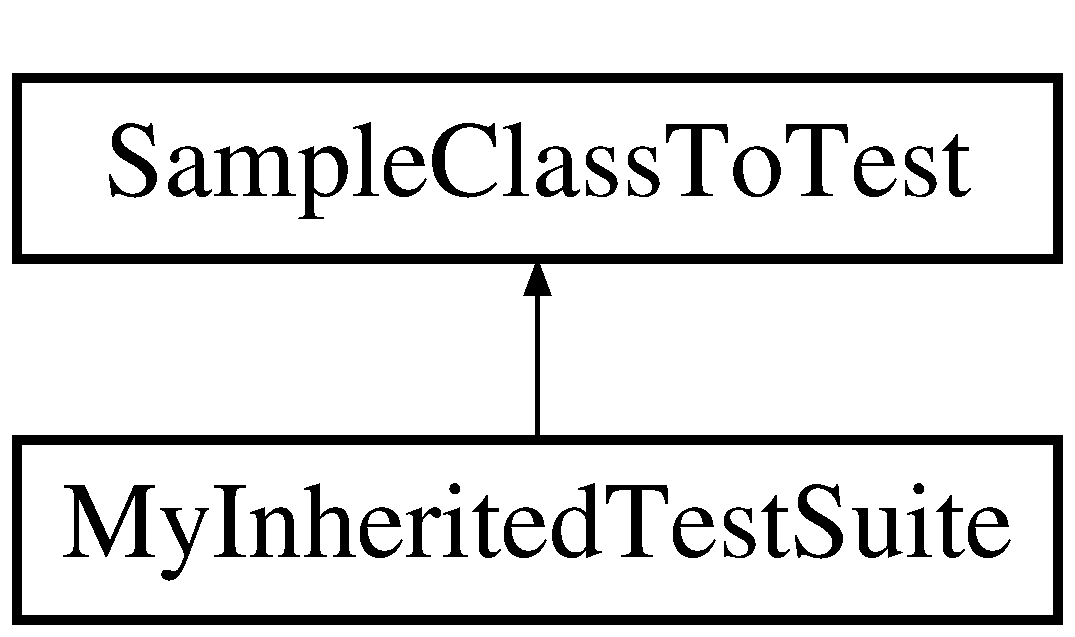
\includegraphics[height=2.000000cm]{class_my_inherited_test_suite}
\end{center}
\end{figure}
\subsection*{Public Member Functions}
\begin{DoxyCompactItemize}
\item 
void \mbox{\hyperlink{class_my_inherited_test_suite_a3aa9d1d4ab762d55cfee1d2f6298c3f9}{set\+Up}} ()
\begin{DoxyCompactList}\small\item\em Initializes each test case. \end{DoxyCompactList}\item 
void \mbox{\hyperlink{class_my_inherited_test_suite_abbd94d1b4868f8252b001ce743eeb691}{tear\+Down}} ()
\begin{DoxyCompactList}\small\item\em Terminate each test case. \end{DoxyCompactList}\item 
void \mbox{\hyperlink{class_my_inherited_test_suite_a1a6a926a8fb9d03618008b6d882a1cfe}{test\+\_\+public\+Inherited\+Methods}} ()
\item 
void \mbox{\hyperlink{class_my_inherited_test_suite_a7fef4b3ee5331b5454ce3b6b66813e6d}{test\+\_\+protected\+Inherited\+Methods}} ()
\item 
void \mbox{\hyperlink{class_my_inherited_test_suite_a17797338b2152e4c8d5354f2efd30692}{test\+\_\+private\+Inherited\+Methods}} ()
\end{DoxyCompactItemize}
\subsection*{Additional Inherited Members}


\subsection{Detailed Description}
Example of Test Suite. 

Run some tests inherited from a parent class 

Definition at line 207 of file Basic\+Test\+Suite\+\_\+\+Test.\+mqh.



\subsection{Member Function Documentation}
\mbox{\Hypertarget{class_my_inherited_test_suite_a3aa9d1d4ab762d55cfee1d2f6298c3f9}\label{class_my_inherited_test_suite_a3aa9d1d4ab762d55cfee1d2f6298c3f9}} 
\index{My\+Inherited\+Test\+Suite@{My\+Inherited\+Test\+Suite}!set\+Up@{set\+Up}}
\index{set\+Up@{set\+Up}!My\+Inherited\+Test\+Suite@{My\+Inherited\+Test\+Suite}}
\subsubsection{\texorpdfstring{set\+Up()}{setUp()}}
{\footnotesize\ttfamily void My\+Inherited\+Test\+Suite\+::set\+Up (\begin{DoxyParamCaption}{ }\end{DoxyParamCaption})\hspace{0.3cm}{\ttfamily [inline]}}



Initializes each test case. 

This is called before each test case runs 

Definition at line 214 of file Basic\+Test\+Suite\+\_\+\+Test.\+mqh.

\mbox{\Hypertarget{class_my_inherited_test_suite_abbd94d1b4868f8252b001ce743eeb691}\label{class_my_inherited_test_suite_abbd94d1b4868f8252b001ce743eeb691}} 
\index{My\+Inherited\+Test\+Suite@{My\+Inherited\+Test\+Suite}!tear\+Down@{tear\+Down}}
\index{tear\+Down@{tear\+Down}!My\+Inherited\+Test\+Suite@{My\+Inherited\+Test\+Suite}}
\subsubsection{\texorpdfstring{tear\+Down()}{tearDown()}}
{\footnotesize\ttfamily void My\+Inherited\+Test\+Suite\+::tear\+Down (\begin{DoxyParamCaption}{ }\end{DoxyParamCaption})\hspace{0.3cm}{\ttfamily [inline]}}



Terminate each test case. 

This is called after each test case runs 

Definition at line 221 of file Basic\+Test\+Suite\+\_\+\+Test.\+mqh.

\mbox{\Hypertarget{class_my_inherited_test_suite_a17797338b2152e4c8d5354f2efd30692}\label{class_my_inherited_test_suite_a17797338b2152e4c8d5354f2efd30692}} 
\index{My\+Inherited\+Test\+Suite@{My\+Inherited\+Test\+Suite}!test\+\_\+private\+Inherited\+Methods@{test\+\_\+private\+Inherited\+Methods}}
\index{test\+\_\+private\+Inherited\+Methods@{test\+\_\+private\+Inherited\+Methods}!My\+Inherited\+Test\+Suite@{My\+Inherited\+Test\+Suite}}
\subsubsection{\texorpdfstring{test\+\_\+private\+Inherited\+Methods()}{test\_privateInheritedMethods()}}
{\footnotesize\ttfamily void My\+Inherited\+Test\+Suite\+::test\+\_\+private\+Inherited\+Methods (\begin{DoxyParamCaption}{ }\end{DoxyParamCaption})\hspace{0.3cm}{\ttfamily [inline]}}



Definition at line 235 of file Basic\+Test\+Suite\+\_\+\+Test.\+mqh.

\mbox{\Hypertarget{class_my_inherited_test_suite_a7fef4b3ee5331b5454ce3b6b66813e6d}\label{class_my_inherited_test_suite_a7fef4b3ee5331b5454ce3b6b66813e6d}} 
\index{My\+Inherited\+Test\+Suite@{My\+Inherited\+Test\+Suite}!test\+\_\+protected\+Inherited\+Methods@{test\+\_\+protected\+Inherited\+Methods}}
\index{test\+\_\+protected\+Inherited\+Methods@{test\+\_\+protected\+Inherited\+Methods}!My\+Inherited\+Test\+Suite@{My\+Inherited\+Test\+Suite}}
\subsubsection{\texorpdfstring{test\+\_\+protected\+Inherited\+Methods()}{test\_protectedInheritedMethods()}}
{\footnotesize\ttfamily void My\+Inherited\+Test\+Suite\+::test\+\_\+protected\+Inherited\+Methods (\begin{DoxyParamCaption}{ }\end{DoxyParamCaption})\hspace{0.3cm}{\ttfamily [inline]}}



Definition at line 230 of file Basic\+Test\+Suite\+\_\+\+Test.\+mqh.

\mbox{\Hypertarget{class_my_inherited_test_suite_a1a6a926a8fb9d03618008b6d882a1cfe}\label{class_my_inherited_test_suite_a1a6a926a8fb9d03618008b6d882a1cfe}} 
\index{My\+Inherited\+Test\+Suite@{My\+Inherited\+Test\+Suite}!test\+\_\+public\+Inherited\+Methods@{test\+\_\+public\+Inherited\+Methods}}
\index{test\+\_\+public\+Inherited\+Methods@{test\+\_\+public\+Inherited\+Methods}!My\+Inherited\+Test\+Suite@{My\+Inherited\+Test\+Suite}}
\subsubsection{\texorpdfstring{test\+\_\+public\+Inherited\+Methods()}{test\_publicInheritedMethods()}}
{\footnotesize\ttfamily void My\+Inherited\+Test\+Suite\+::test\+\_\+public\+Inherited\+Methods (\begin{DoxyParamCaption}{ }\end{DoxyParamCaption})\hspace{0.3cm}{\ttfamily [inline]}}



Definition at line 225 of file Basic\+Test\+Suite\+\_\+\+Test.\+mqh.



The documentation for this class was generated from the following file\+:\begin{DoxyCompactItemize}
\item 
C\+:/\+Program Files/\+Meta\+Trader 5/\+M\+Q\+L5/\+Experts/\+My\+Unit\+Test\+E\+A/\+Test/\mbox{\hyperlink{_basic_test_suite___test_8mqh}{Basic\+Test\+Suite\+\_\+\+Test.\+mqh}}\end{DoxyCompactItemize}

\hypertarget{class_sample_class_to_test}{}\section{Sample\+Class\+To\+Test Class Reference}
\label{class_sample_class_to_test}\index{Sample\+Class\+To\+Test@{Sample\+Class\+To\+Test}}
Inheritance diagram for Sample\+Class\+To\+Test\+:\begin{figure}[H]
\begin{center}
\leavevmode
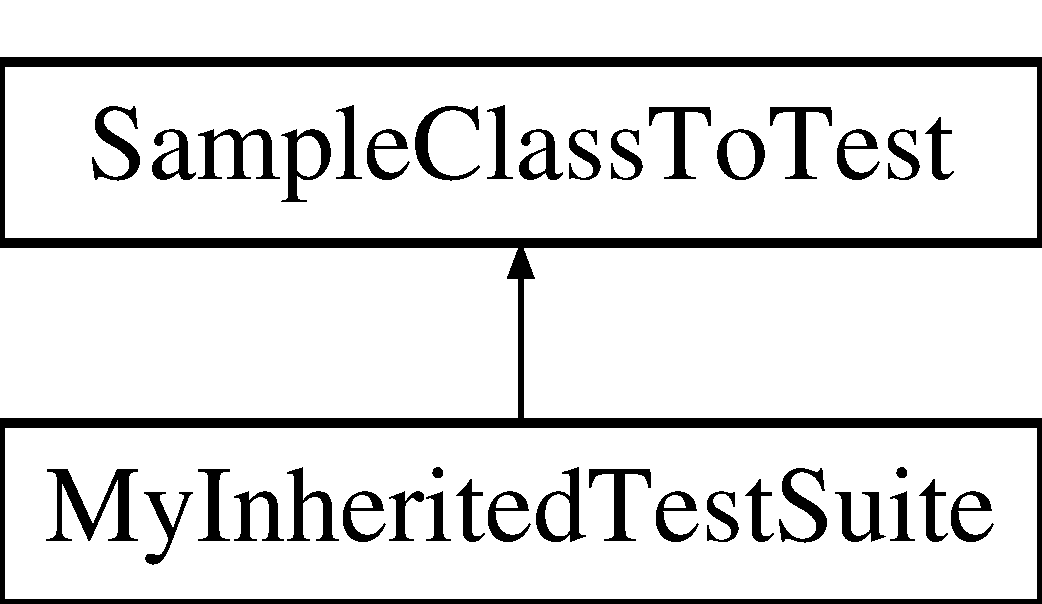
\includegraphics[height=2.000000cm]{class_sample_class_to_test}
\end{center}
\end{figure}
\subsection*{Public Member Functions}
\begin{DoxyCompactItemize}
\item 
\mbox{\hyperlink{class_sample_class_to_test_ab3aa0ae3270fcfbe452c8584533dadb3}{Sample\+Class\+To\+Test}} ()
\item 
\mbox{\hyperlink{class_sample_class_to_test_ab1e66b62ca5dc130dbd50ea3d9aea373}{$\sim$\+Sample\+Class\+To\+Test}} ()
\item 
bool \mbox{\hyperlink{class_sample_class_to_test_a0cb90e0d767aa37ce85fe9042c5a1ad1}{sample\+Public\+Method}} ()
\item 
bool \mbox{\hyperlink{class_sample_class_to_test_a0d019a65a59ccaddca38a1c20036929d}{sample\+Public\+Method\+To\+Test\+Private\+Methods}} ()
\end{DoxyCompactItemize}
\subsection*{Static Public Member Functions}
\begin{DoxyCompactItemize}
\item 
static bool \mbox{\hyperlink{class_sample_class_to_test_a7dcee5d64f6d25294e17e68939a039d4}{sample\+Static\+Method}} ()
\end{DoxyCompactItemize}
\subsection*{Protected Member Functions}
\begin{DoxyCompactItemize}
\item 
bool \mbox{\hyperlink{class_sample_class_to_test_aabb7ee2f669ca4fa7e89b62267742b81}{sample\+Protected\+Method}} ()
\item 
bool \mbox{\hyperlink{class_sample_class_to_test_a84a45488260409b10a2fc95cf0f079b8}{sample\+Protected\+Method\+To\+Test\+Private\+Methods}} ()
\end{DoxyCompactItemize}


\subsection{Detailed Description}


Definition at line 14 of file Sample\+Class\+To\+Test.\+mqh.



\subsection{Constructor \& Destructor Documentation}
\mbox{\Hypertarget{class_sample_class_to_test_ab3aa0ae3270fcfbe452c8584533dadb3}\label{class_sample_class_to_test_ab3aa0ae3270fcfbe452c8584533dadb3}} 
\index{Sample\+Class\+To\+Test@{Sample\+Class\+To\+Test}!Sample\+Class\+To\+Test@{Sample\+Class\+To\+Test}}
\index{Sample\+Class\+To\+Test@{Sample\+Class\+To\+Test}!Sample\+Class\+To\+Test@{Sample\+Class\+To\+Test}}
\subsubsection{\texorpdfstring{Sample\+Class\+To\+Test()}{SampleClassToTest()}}
{\footnotesize\ttfamily Sample\+Class\+To\+Test\+::\+Sample\+Class\+To\+Test (\begin{DoxyParamCaption}{ }\end{DoxyParamCaption})\hspace{0.3cm}{\ttfamily [inline]}}



Definition at line 17 of file Sample\+Class\+To\+Test.\+mqh.

\mbox{\Hypertarget{class_sample_class_to_test_ab1e66b62ca5dc130dbd50ea3d9aea373}\label{class_sample_class_to_test_ab1e66b62ca5dc130dbd50ea3d9aea373}} 
\index{Sample\+Class\+To\+Test@{Sample\+Class\+To\+Test}!````~Sample\+Class\+To\+Test@{$\sim$\+Sample\+Class\+To\+Test}}
\index{````~Sample\+Class\+To\+Test@{$\sim$\+Sample\+Class\+To\+Test}!Sample\+Class\+To\+Test@{Sample\+Class\+To\+Test}}
\subsubsection{\texorpdfstring{$\sim$\+Sample\+Class\+To\+Test()}{~SampleClassToTest()}}
{\footnotesize\ttfamily Sample\+Class\+To\+Test\+::$\sim$\+Sample\+Class\+To\+Test (\begin{DoxyParamCaption}{ }\end{DoxyParamCaption})\hspace{0.3cm}{\ttfamily [inline]}}



Definition at line 18 of file Sample\+Class\+To\+Test.\+mqh.



\subsection{Member Function Documentation}
\mbox{\Hypertarget{class_sample_class_to_test_aabb7ee2f669ca4fa7e89b62267742b81}\label{class_sample_class_to_test_aabb7ee2f669ca4fa7e89b62267742b81}} 
\index{Sample\+Class\+To\+Test@{Sample\+Class\+To\+Test}!sample\+Protected\+Method@{sample\+Protected\+Method}}
\index{sample\+Protected\+Method@{sample\+Protected\+Method}!Sample\+Class\+To\+Test@{Sample\+Class\+To\+Test}}
\subsubsection{\texorpdfstring{sample\+Protected\+Method()}{sampleProtectedMethod()}}
{\footnotesize\ttfamily bool Sample\+Class\+To\+Test\+::sample\+Protected\+Method (\begin{DoxyParamCaption}{ }\end{DoxyParamCaption})\hspace{0.3cm}{\ttfamily [inline]}, {\ttfamily [protected]}}



Definition at line 35 of file Sample\+Class\+To\+Test.\+mqh.

\mbox{\Hypertarget{class_sample_class_to_test_a84a45488260409b10a2fc95cf0f079b8}\label{class_sample_class_to_test_a84a45488260409b10a2fc95cf0f079b8}} 
\index{Sample\+Class\+To\+Test@{Sample\+Class\+To\+Test}!sample\+Protected\+Method\+To\+Test\+Private\+Methods@{sample\+Protected\+Method\+To\+Test\+Private\+Methods}}
\index{sample\+Protected\+Method\+To\+Test\+Private\+Methods@{sample\+Protected\+Method\+To\+Test\+Private\+Methods}!Sample\+Class\+To\+Test@{Sample\+Class\+To\+Test}}
\subsubsection{\texorpdfstring{sample\+Protected\+Method\+To\+Test\+Private\+Methods()}{sampleProtectedMethodToTestPrivateMethods()}}
{\footnotesize\ttfamily bool Sample\+Class\+To\+Test\+::sample\+Protected\+Method\+To\+Test\+Private\+Methods (\begin{DoxyParamCaption}{ }\end{DoxyParamCaption})\hspace{0.3cm}{\ttfamily [inline]}, {\ttfamily [protected]}}



Definition at line 40 of file Sample\+Class\+To\+Test.\+mqh.

\mbox{\Hypertarget{class_sample_class_to_test_a0cb90e0d767aa37ce85fe9042c5a1ad1}\label{class_sample_class_to_test_a0cb90e0d767aa37ce85fe9042c5a1ad1}} 
\index{Sample\+Class\+To\+Test@{Sample\+Class\+To\+Test}!sample\+Public\+Method@{sample\+Public\+Method}}
\index{sample\+Public\+Method@{sample\+Public\+Method}!Sample\+Class\+To\+Test@{Sample\+Class\+To\+Test}}
\subsubsection{\texorpdfstring{sample\+Public\+Method()}{samplePublicMethod()}}
{\footnotesize\ttfamily bool Sample\+Class\+To\+Test\+::sample\+Public\+Method (\begin{DoxyParamCaption}{ }\end{DoxyParamCaption})\hspace{0.3cm}{\ttfamily [inline]}}



Definition at line 19 of file Sample\+Class\+To\+Test.\+mqh.

\mbox{\Hypertarget{class_sample_class_to_test_a0d019a65a59ccaddca38a1c20036929d}\label{class_sample_class_to_test_a0d019a65a59ccaddca38a1c20036929d}} 
\index{Sample\+Class\+To\+Test@{Sample\+Class\+To\+Test}!sample\+Public\+Method\+To\+Test\+Private\+Methods@{sample\+Public\+Method\+To\+Test\+Private\+Methods}}
\index{sample\+Public\+Method\+To\+Test\+Private\+Methods@{sample\+Public\+Method\+To\+Test\+Private\+Methods}!Sample\+Class\+To\+Test@{Sample\+Class\+To\+Test}}
\subsubsection{\texorpdfstring{sample\+Public\+Method\+To\+Test\+Private\+Methods()}{samplePublicMethodToTestPrivateMethods()}}
{\footnotesize\ttfamily bool Sample\+Class\+To\+Test\+::sample\+Public\+Method\+To\+Test\+Private\+Methods (\begin{DoxyParamCaption}{ }\end{DoxyParamCaption})\hspace{0.3cm}{\ttfamily [inline]}}



Definition at line 29 of file Sample\+Class\+To\+Test.\+mqh.

\mbox{\Hypertarget{class_sample_class_to_test_a7dcee5d64f6d25294e17e68939a039d4}\label{class_sample_class_to_test_a7dcee5d64f6d25294e17e68939a039d4}} 
\index{Sample\+Class\+To\+Test@{Sample\+Class\+To\+Test}!sample\+Static\+Method@{sample\+Static\+Method}}
\index{sample\+Static\+Method@{sample\+Static\+Method}!Sample\+Class\+To\+Test@{Sample\+Class\+To\+Test}}
\subsubsection{\texorpdfstring{sample\+Static\+Method()}{sampleStaticMethod()}}
{\footnotesize\ttfamily static bool Sample\+Class\+To\+Test\+::sample\+Static\+Method (\begin{DoxyParamCaption}{ }\end{DoxyParamCaption})\hspace{0.3cm}{\ttfamily [inline]}, {\ttfamily [static]}}



Definition at line 24 of file Sample\+Class\+To\+Test.\+mqh.



The documentation for this class was generated from the following file\+:\begin{DoxyCompactItemize}
\item 
C\+:/\+Program Files/\+Meta\+Trader 5/\+M\+Q\+L5/\+Experts/\+My\+Unit\+Test\+E\+A/\+Include/\mbox{\hyperlink{_sample_class_to_test_8mqh}{Sample\+Class\+To\+Test.\+mqh}}\end{DoxyCompactItemize}

\chapter{File Documentation}
\hypertarget{_my_unit_test_e_a_8mq5}{}\section{My\+Unit\+Test\+E\+A.\+mq5 File Reference}
\label{_my_unit_test_e_a_8mq5}\index{My\+Unit\+Test\+E\+A.\+mq5@{My\+Unit\+Test\+E\+A.\+mq5}}


This file represents an Expert Advisor capable of running our Test Unit. It also demonstrates how to use it properly.  


{\ttfamily \#include \char`\"{}../\+Include/\+M\+T\+Unit.\+mqh\char`\"{}}\newline
\subsection*{Functions}
\begin{DoxyCompactItemize}
\item 
int \mbox{\hyperlink{_my_unit_test_e_a_8mq5_a53dc1cd6aabfadddd579c1b1010e7d52}{On\+Init}} ()
\begin{DoxyCompactList}\small\item\em Expert On\+Init function. \end{DoxyCompactList}\item 
void \mbox{\hyperlink{_my_unit_test_e_a_8mq5_a3f95d0fb3935a6dd3f45618a48fea55b}{On\+Deinit}} (const int reason)
\begin{DoxyCompactList}\small\item\em Expert On\+Deinit function. \end{DoxyCompactList}\item 
void \mbox{\hyperlink{_my_unit_test_e_a_8mq5_a94383cb2b73d2bc8d5536e293232374f}{On\+Tick}} ()
\begin{DoxyCompactList}\small\item\em Expert tick function {\itshape D\+I\+S\+A\+B\+L\+ED} \end{DoxyCompactList}\item 
double \mbox{\hyperlink{_my_unit_test_e_a_8mq5_a7b3651ef0dea162e4f2217474bf878aa}{get\+MA}} (int shift)
\item 
void \mbox{\hyperlink{_my_unit_test_e_a_8mq5_a2522426d9de7bcd6c5348e9e2835b36d}{get\+M\+A\+Array}} (const int \&shifts\mbox{[}$\,$\mbox{]}, double \&mas\mbox{[}$\,$\mbox{]})
\end{DoxyCompactItemize}


\subsection{Detailed Description}
This file represents an Expert Advisor capable of running our Test Unit. It also demonstrates how to use it properly. 

\begin{DoxyAuthor}{Author}
Rodrigo Haller 
\end{DoxyAuthor}
\begin{DoxyDate}{Date}
09/02/2018 
\end{DoxyDate}


\subsection{Function Documentation}
\mbox{\Hypertarget{_my_unit_test_e_a_8mq5_a7b3651ef0dea162e4f2217474bf878aa}\label{_my_unit_test_e_a_8mq5_a7b3651ef0dea162e4f2217474bf878aa}} 
\index{My\+Unit\+Test\+E\+A.\+mq5@{My\+Unit\+Test\+E\+A.\+mq5}!get\+MA@{get\+MA}}
\index{get\+MA@{get\+MA}!My\+Unit\+Test\+E\+A.\+mq5@{My\+Unit\+Test\+E\+A.\+mq5}}
\subsubsection{\texorpdfstring{get\+M\+A()}{getMA()}}
{\footnotesize\ttfamily double get\+MA (\begin{DoxyParamCaption}\item[{int}]{shift }\end{DoxyParamCaption})}



Definition at line 54 of file My\+Unit\+Test\+E\+A.\+mq5.

\mbox{\Hypertarget{_my_unit_test_e_a_8mq5_a2522426d9de7bcd6c5348e9e2835b36d}\label{_my_unit_test_e_a_8mq5_a2522426d9de7bcd6c5348e9e2835b36d}} 
\index{My\+Unit\+Test\+E\+A.\+mq5@{My\+Unit\+Test\+E\+A.\+mq5}!get\+M\+A\+Array@{get\+M\+A\+Array}}
\index{get\+M\+A\+Array@{get\+M\+A\+Array}!My\+Unit\+Test\+E\+A.\+mq5@{My\+Unit\+Test\+E\+A.\+mq5}}
\subsubsection{\texorpdfstring{get\+M\+A\+Array()}{getMAArray()}}
{\footnotesize\ttfamily void get\+M\+A\+Array (\begin{DoxyParamCaption}\item[{const int \&}]{shifts\mbox{[}$\,$\mbox{]},  }\item[{double \&}]{mas\mbox{[}$\,$\mbox{]} }\end{DoxyParamCaption})}



Definition at line 59 of file My\+Unit\+Test\+E\+A.\+mq5.

\mbox{\Hypertarget{_my_unit_test_e_a_8mq5_a3f95d0fb3935a6dd3f45618a48fea55b}\label{_my_unit_test_e_a_8mq5_a3f95d0fb3935a6dd3f45618a48fea55b}} 
\index{My\+Unit\+Test\+E\+A.\+mq5@{My\+Unit\+Test\+E\+A.\+mq5}!On\+Deinit@{On\+Deinit}}
\index{On\+Deinit@{On\+Deinit}!My\+Unit\+Test\+E\+A.\+mq5@{My\+Unit\+Test\+E\+A.\+mq5}}
\subsubsection{\texorpdfstring{On\+Deinit()}{OnDeinit()}}
{\footnotesize\ttfamily void On\+Deinit (\begin{DoxyParamCaption}\item[{const int}]{reason }\end{DoxyParamCaption})}



Expert On\+Deinit function. 

Call U\+T\+\_\+\+On\+De\+Init() in your Expert\textquotesingle{}s \mbox{\hyperlink{_my_unit_test_e_a_8mq5_a3f95d0fb3935a6dd3f45618a48fea55b}{On\+Deinit()}} method to delete the Unit\+Test objects. 

Definition at line 32 of file My\+Unit\+Test\+E\+A.\+mq5.

\mbox{\Hypertarget{_my_unit_test_e_a_8mq5_a53dc1cd6aabfadddd579c1b1010e7d52}\label{_my_unit_test_e_a_8mq5_a53dc1cd6aabfadddd579c1b1010e7d52}} 
\index{My\+Unit\+Test\+E\+A.\+mq5@{My\+Unit\+Test\+E\+A.\+mq5}!On\+Init@{On\+Init}}
\index{On\+Init@{On\+Init}!My\+Unit\+Test\+E\+A.\+mq5@{My\+Unit\+Test\+E\+A.\+mq5}}
\subsubsection{\texorpdfstring{On\+Init()}{OnInit()}}
{\footnotesize\ttfamily int On\+Init (\begin{DoxyParamCaption}{ }\end{DoxyParamCaption})}



Expert On\+Init function. 

Call \mbox{\hyperlink{_m_t_unit_8mqh_a9cdc57544d91884fab6f627b3394326f}{U\+T\+\_\+\+On\+Init()}} in your Expert\textquotesingle{}s \mbox{\hyperlink{_my_unit_test_e_a_8mq5_a53dc1cd6aabfadddd579c1b1010e7d52}{On\+Init()}} method to run the tests. \begin{DoxyReturn}{Returns}
Expert return status 
\end{DoxyReturn}


Definition at line 21 of file My\+Unit\+Test\+E\+A.\+mq5.

\mbox{\Hypertarget{_my_unit_test_e_a_8mq5_a94383cb2b73d2bc8d5536e293232374f}\label{_my_unit_test_e_a_8mq5_a94383cb2b73d2bc8d5536e293232374f}} 
\index{My\+Unit\+Test\+E\+A.\+mq5@{My\+Unit\+Test\+E\+A.\+mq5}!On\+Tick@{On\+Tick}}
\index{On\+Tick@{On\+Tick}!My\+Unit\+Test\+E\+A.\+mq5@{My\+Unit\+Test\+E\+A.\+mq5}}
\subsubsection{\texorpdfstring{On\+Tick()}{OnTick()}}
{\footnotesize\ttfamily void On\+Tick (\begin{DoxyParamCaption}{ }\end{DoxyParamCaption})}



Expert tick function {\itshape D\+I\+S\+A\+B\+L\+ED} 

Not commonly used, but if you have tests that should run on each Tick, call \mbox{\hyperlink{_m_t_unit_8mqh_afcdc18c227067029c1bb10f935bdb21c}{U\+T\+\_\+\+On\+Tick()}}. \begin{DoxyWarning}{Warning}
Do not forget to set g\+\_\+unit\+Testing\+On\+Tick to true 
\end{DoxyWarning}
\begin{DoxyNote}{Note}
This option is disabled for now, since I don\textquotesingle{}t see any use for this. Unit\+Tests should not rely on random data, that\textquotesingle{}s why mocking objects exist. So I don\textquotesingle{}t see the point of testing during ticks. 
\end{DoxyNote}


Definition at line 47 of file My\+Unit\+Test\+E\+A.\+mq5.


\hypertarget{_m_t_unit_8mqh}{}\section{C\+:/\+Program Files/\+Meta\+Trader 5/\+M\+Q\+L5/\+Experts/\+My\+Unit\+Test\+E\+A/\+Include/\+M\+T\+Unit.mqh File Reference}
\label{_m_t_unit_8mqh}\index{C\+:/\+Program Files/\+Meta\+Trader 5/\+M\+Q\+L5/\+Experts/\+My\+Unit\+Test\+E\+A/\+Include/\+M\+T\+Unit.\+mqh@{C\+:/\+Program Files/\+Meta\+Trader 5/\+M\+Q\+L5/\+Experts/\+My\+Unit\+Test\+E\+A/\+Include/\+M\+T\+Unit.\+mqh}}


File containing a Unit Test library developed for M\+Q\+L5 This file was based on this article\+: \href{https://www.mql5.com/ru/articles/1579}{\tt https\+://www.\+mql5.\+com/ru/articles/1579}.  


{\ttfamily \#include \char`\"{}M\+T\+Unit\+Cfg.\+mqh\char`\"{}}\newline
{\ttfamily \#include \char`\"{}M\+T\+Unit\+All\+Tests.\+mqh\char`\"{}}\newline
\subsection*{Classes}
\begin{DoxyCompactItemize}
\item 
class \mbox{\hyperlink{class_m_t_unit}{M\+T\+Unit}}
\end{DoxyCompactItemize}
\subsection*{Macros}
\begin{DoxyCompactItemize}
\item 
\#define \mbox{\hyperlink{_m_t_unit_8mqh_abec0187655f13dec59b96cde105e5bc1}{U\+T\+\_\+\+S\+P\+A\+C\+E\+\_\+\+T\+E\+S\+T\+C\+A\+SE}}~\char`\"{}  \char`\"{}
\item 
\#define \mbox{\hyperlink{_m_t_unit_8mqh_a41d9aa881079f30c8488682ba6a90014}{U\+T\+\_\+\+S\+P\+A\+C\+E\+\_\+\+A\+S\+S\+E\+RT}}~\char`\"{}\mbox{[}T\+E\+ST\mbox{]} \char`\"{}
\item 
\#define \mbox{\hyperlink{_m_t_unit_8mqh_a4631b5eea3d8e74cd319ef46940fb539}{U\+T\+\_\+\+S\+EP}}~\char`\"{} -\/ \char`\"{}
\item 
\#define \mbox{\hyperlink{_m_t_unit_8mqh_a6369f0c6469a39ec1afa8834e8a96733}{U\+T\+\_\+\+C\+O\+M\+P\+\_\+\+E\+X\+P\+\_\+\+A\+CT}}~\char`\"{}\%s\+: expected is $<$\%s$>$ but $<$\%s$>$\char`\"{}
\item 
\#define \mbox{\hyperlink{_m_t_unit_8mqh_afdcc024902d14669b7a22158e646299b}{U\+T\+\_\+\+C\+O\+M\+P\+\_\+\+A\+R\+R\+\_\+\+E\+X\+P\+\_\+\+A\+CT}}~\char`\"{}\%s\+: expected array\mbox{[}\%d\mbox{]} is $<$\%s$>$ but $<$\%s$>$\char`\"{}
\item 
\#define \mbox{\hyperlink{_m_t_unit_8mqh_a96f5d62188d09039ebc3f443c9120e39}{U\+T\+\_\+\+D\+E\+F\+A\+U\+L\+T\+\_\+\+A\+S\+S\+E\+R\+T\+\_\+\+M\+E\+S\+S\+A\+GE}}~\char`\"{}Assert should succeed\char`\"{}
\end{DoxyCompactItemize}
\subsection*{Functions}
\begin{DoxyCompactItemize}
\item 
void \mbox{\hyperlink{_m_t_unit_8mqh_a9cdc57544d91884fab6f627b3394326f}{U\+T\+\_\+\+On\+Init}} ()
\begin{DoxyCompactList}\small\item\em On\+Init method of the \mbox{\hyperlink{class_m_t_unit}{M\+T\+Unit}}. \end{DoxyCompactList}\item 
void \mbox{\hyperlink{_m_t_unit_8mqh_a9fbaaa20ba4e1624e348f7ab5109ecbf}{U\+T\+\_\+\+On\+Deinit}} ()
\item 
void \mbox{\hyperlink{_m_t_unit_8mqh_afcdc18c227067029c1bb10f935bdb21c}{U\+T\+\_\+\+On\+Tick}} ()
\item 
string \mbox{\hyperlink{_m_t_unit_8mqh_a560d9b8bdbe896abd079b6c9d7bd107f}{get\+O\+K\+Fail}} (bool ok)
\item 
string \mbox{\hyperlink{_m_t_unit_8mqh_a846b4d0b246628bc40f57371459bdf2f}{bool\+To\+String}} (bool b)
\end{DoxyCompactItemize}
\subsection*{Variables}
\begin{DoxyCompactItemize}
\item 
\mbox{\hyperlink{class_m_t_unit}{M\+T\+Unit}} $\ast$ \mbox{\hyperlink{_m_t_unit_8mqh_a26846c3d9a3b28dcdfd39654d4527685}{g\+\_\+mt\+Unit}}
\item 
\mbox{\hyperlink{class_m_t_unit_all_tests}{M\+T\+Unit\+All\+Tests}} $\ast$ \mbox{\hyperlink{_m_t_unit_8mqh_af8a46b5767cc8d41db82ddc69eb9f46e}{g\+\_\+mt\+Unit\+All\+Tests}}
\end{DoxyCompactItemize}


\subsection{Detailed Description}
File containing a Unit Test library developed for M\+Q\+L5 This file was based on this article\+: \href{https://www.mql5.com/ru/articles/1579}{\tt https\+://www.\+mql5.\+com/ru/articles/1579}. 

\begin{DoxyAuthor}{Author}
Rodrigo Haller 
\end{DoxyAuthor}
\begin{DoxyDate}{Date}
09/02/2018 
\end{DoxyDate}


\subsection{Macro Definition Documentation}
\mbox{\Hypertarget{_m_t_unit_8mqh_afdcc024902d14669b7a22158e646299b}\label{_m_t_unit_8mqh_afdcc024902d14669b7a22158e646299b}} 
\index{M\+T\+Unit.\+mqh@{M\+T\+Unit.\+mqh}!U\+T\+\_\+\+C\+O\+M\+P\+\_\+\+A\+R\+R\+\_\+\+E\+X\+P\+\_\+\+A\+CT@{U\+T\+\_\+\+C\+O\+M\+P\+\_\+\+A\+R\+R\+\_\+\+E\+X\+P\+\_\+\+A\+CT}}
\index{U\+T\+\_\+\+C\+O\+M\+P\+\_\+\+A\+R\+R\+\_\+\+E\+X\+P\+\_\+\+A\+CT@{U\+T\+\_\+\+C\+O\+M\+P\+\_\+\+A\+R\+R\+\_\+\+E\+X\+P\+\_\+\+A\+CT}!M\+T\+Unit.\+mqh@{M\+T\+Unit.\+mqh}}
\subsubsection{\texorpdfstring{U\+T\+\_\+\+C\+O\+M\+P\+\_\+\+A\+R\+R\+\_\+\+E\+X\+P\+\_\+\+A\+CT}{UT\_COMP\_ARR\_EXP\_ACT}}
{\footnotesize\ttfamily \#define U\+T\+\_\+\+C\+O\+M\+P\+\_\+\+A\+R\+R\+\_\+\+E\+X\+P\+\_\+\+A\+CT~\char`\"{}\%s\+: expected array\mbox{[}\%d\mbox{]} is $<$\%s$>$ but $<$\%s$>$\char`\"{}}



Definition at line 70 of file M\+T\+Unit.\+mqh.

\mbox{\Hypertarget{_m_t_unit_8mqh_a6369f0c6469a39ec1afa8834e8a96733}\label{_m_t_unit_8mqh_a6369f0c6469a39ec1afa8834e8a96733}} 
\index{M\+T\+Unit.\+mqh@{M\+T\+Unit.\+mqh}!U\+T\+\_\+\+C\+O\+M\+P\+\_\+\+E\+X\+P\+\_\+\+A\+CT@{U\+T\+\_\+\+C\+O\+M\+P\+\_\+\+E\+X\+P\+\_\+\+A\+CT}}
\index{U\+T\+\_\+\+C\+O\+M\+P\+\_\+\+E\+X\+P\+\_\+\+A\+CT@{U\+T\+\_\+\+C\+O\+M\+P\+\_\+\+E\+X\+P\+\_\+\+A\+CT}!M\+T\+Unit.\+mqh@{M\+T\+Unit.\+mqh}}
\subsubsection{\texorpdfstring{U\+T\+\_\+\+C\+O\+M\+P\+\_\+\+E\+X\+P\+\_\+\+A\+CT}{UT\_COMP\_EXP\_ACT}}
{\footnotesize\ttfamily \#define U\+T\+\_\+\+C\+O\+M\+P\+\_\+\+E\+X\+P\+\_\+\+A\+CT~\char`\"{}\%s\+: expected is $<$\%s$>$ but $<$\%s$>$\char`\"{}}



Definition at line 69 of file M\+T\+Unit.\+mqh.

\mbox{\Hypertarget{_m_t_unit_8mqh_a96f5d62188d09039ebc3f443c9120e39}\label{_m_t_unit_8mqh_a96f5d62188d09039ebc3f443c9120e39}} 
\index{M\+T\+Unit.\+mqh@{M\+T\+Unit.\+mqh}!U\+T\+\_\+\+D\+E\+F\+A\+U\+L\+T\+\_\+\+A\+S\+S\+E\+R\+T\+\_\+\+M\+E\+S\+S\+A\+GE@{U\+T\+\_\+\+D\+E\+F\+A\+U\+L\+T\+\_\+\+A\+S\+S\+E\+R\+T\+\_\+\+M\+E\+S\+S\+A\+GE}}
\index{U\+T\+\_\+\+D\+E\+F\+A\+U\+L\+T\+\_\+\+A\+S\+S\+E\+R\+T\+\_\+\+M\+E\+S\+S\+A\+GE@{U\+T\+\_\+\+D\+E\+F\+A\+U\+L\+T\+\_\+\+A\+S\+S\+E\+R\+T\+\_\+\+M\+E\+S\+S\+A\+GE}!M\+T\+Unit.\+mqh@{M\+T\+Unit.\+mqh}}
\subsubsection{\texorpdfstring{U\+T\+\_\+\+D\+E\+F\+A\+U\+L\+T\+\_\+\+A\+S\+S\+E\+R\+T\+\_\+\+M\+E\+S\+S\+A\+GE}{UT\_DEFAULT\_ASSERT\_MESSAGE}}
{\footnotesize\ttfamily \#define U\+T\+\_\+\+D\+E\+F\+A\+U\+L\+T\+\_\+\+A\+S\+S\+E\+R\+T\+\_\+\+M\+E\+S\+S\+A\+GE~\char`\"{}Assert should succeed\char`\"{}}



Definition at line 71 of file M\+T\+Unit.\+mqh.

\mbox{\Hypertarget{_m_t_unit_8mqh_a4631b5eea3d8e74cd319ef46940fb539}\label{_m_t_unit_8mqh_a4631b5eea3d8e74cd319ef46940fb539}} 
\index{M\+T\+Unit.\+mqh@{M\+T\+Unit.\+mqh}!U\+T\+\_\+\+S\+EP@{U\+T\+\_\+\+S\+EP}}
\index{U\+T\+\_\+\+S\+EP@{U\+T\+\_\+\+S\+EP}!M\+T\+Unit.\+mqh@{M\+T\+Unit.\+mqh}}
\subsubsection{\texorpdfstring{U\+T\+\_\+\+S\+EP}{UT\_SEP}}
{\footnotesize\ttfamily \#define U\+T\+\_\+\+S\+EP~\char`\"{} -\/ \char`\"{}}



Definition at line 68 of file M\+T\+Unit.\+mqh.

\mbox{\Hypertarget{_m_t_unit_8mqh_a41d9aa881079f30c8488682ba6a90014}\label{_m_t_unit_8mqh_a41d9aa881079f30c8488682ba6a90014}} 
\index{M\+T\+Unit.\+mqh@{M\+T\+Unit.\+mqh}!U\+T\+\_\+\+S\+P\+A\+C\+E\+\_\+\+A\+S\+S\+E\+RT@{U\+T\+\_\+\+S\+P\+A\+C\+E\+\_\+\+A\+S\+S\+E\+RT}}
\index{U\+T\+\_\+\+S\+P\+A\+C\+E\+\_\+\+A\+S\+S\+E\+RT@{U\+T\+\_\+\+S\+P\+A\+C\+E\+\_\+\+A\+S\+S\+E\+RT}!M\+T\+Unit.\+mqh@{M\+T\+Unit.\+mqh}}
\subsubsection{\texorpdfstring{U\+T\+\_\+\+S\+P\+A\+C\+E\+\_\+\+A\+S\+S\+E\+RT}{UT\_SPACE\_ASSERT}}
{\footnotesize\ttfamily \#define U\+T\+\_\+\+S\+P\+A\+C\+E\+\_\+\+A\+S\+S\+E\+RT~\char`\"{}\mbox{[}T\+E\+ST\mbox{]} \char`\"{}}



Definition at line 67 of file M\+T\+Unit.\+mqh.

\mbox{\Hypertarget{_m_t_unit_8mqh_abec0187655f13dec59b96cde105e5bc1}\label{_m_t_unit_8mqh_abec0187655f13dec59b96cde105e5bc1}} 
\index{M\+T\+Unit.\+mqh@{M\+T\+Unit.\+mqh}!U\+T\+\_\+\+S\+P\+A\+C\+E\+\_\+\+T\+E\+S\+T\+C\+A\+SE@{U\+T\+\_\+\+S\+P\+A\+C\+E\+\_\+\+T\+E\+S\+T\+C\+A\+SE}}
\index{U\+T\+\_\+\+S\+P\+A\+C\+E\+\_\+\+T\+E\+S\+T\+C\+A\+SE@{U\+T\+\_\+\+S\+P\+A\+C\+E\+\_\+\+T\+E\+S\+T\+C\+A\+SE}!M\+T\+Unit.\+mqh@{M\+T\+Unit.\+mqh}}
\subsubsection{\texorpdfstring{U\+T\+\_\+\+S\+P\+A\+C\+E\+\_\+\+T\+E\+S\+T\+C\+A\+SE}{UT\_SPACE\_TESTCASE}}
{\footnotesize\ttfamily \#define U\+T\+\_\+\+S\+P\+A\+C\+E\+\_\+\+T\+E\+S\+T\+C\+A\+SE~\char`\"{}  \char`\"{}}



Definition at line 66 of file M\+T\+Unit.\+mqh.



\subsection{Function Documentation}
\mbox{\Hypertarget{_m_t_unit_8mqh_a846b4d0b246628bc40f57371459bdf2f}\label{_m_t_unit_8mqh_a846b4d0b246628bc40f57371459bdf2f}} 
\index{M\+T\+Unit.\+mqh@{M\+T\+Unit.\+mqh}!bool\+To\+String@{bool\+To\+String}}
\index{bool\+To\+String@{bool\+To\+String}!M\+T\+Unit.\+mqh@{M\+T\+Unit.\+mqh}}
\subsubsection{\texorpdfstring{bool\+To\+String()}{boolToString()}}
{\footnotesize\ttfamily string bool\+To\+String (\begin{DoxyParamCaption}\item[{bool}]{b }\end{DoxyParamCaption})}



Definition at line 830 of file M\+T\+Unit.\+mqh.

\mbox{\Hypertarget{_m_t_unit_8mqh_a560d9b8bdbe896abd079b6c9d7bd107f}\label{_m_t_unit_8mqh_a560d9b8bdbe896abd079b6c9d7bd107f}} 
\index{M\+T\+Unit.\+mqh@{M\+T\+Unit.\+mqh}!get\+O\+K\+Fail@{get\+O\+K\+Fail}}
\index{get\+O\+K\+Fail@{get\+O\+K\+Fail}!M\+T\+Unit.\+mqh@{M\+T\+Unit.\+mqh}}
\subsubsection{\texorpdfstring{get\+O\+K\+Fail()}{getOKFail()}}
{\footnotesize\ttfamily string get\+O\+K\+Fail (\begin{DoxyParamCaption}\item[{bool}]{ok }\end{DoxyParamCaption})}



Definition at line 294 of file M\+T\+Unit.\+mqh.

\mbox{\Hypertarget{_m_t_unit_8mqh_a9fbaaa20ba4e1624e348f7ab5109ecbf}\label{_m_t_unit_8mqh_a9fbaaa20ba4e1624e348f7ab5109ecbf}} 
\index{M\+T\+Unit.\+mqh@{M\+T\+Unit.\+mqh}!U\+T\+\_\+\+On\+Deinit@{U\+T\+\_\+\+On\+Deinit}}
\index{U\+T\+\_\+\+On\+Deinit@{U\+T\+\_\+\+On\+Deinit}!M\+T\+Unit.\+mqh@{M\+T\+Unit.\+mqh}}
\subsubsection{\texorpdfstring{U\+T\+\_\+\+On\+Deinit()}{UT\_OnDeinit()}}
{\footnotesize\ttfamily void U\+T\+\_\+\+On\+Deinit (\begin{DoxyParamCaption}{ }\end{DoxyParamCaption})}



Definition at line 53 of file M\+T\+Unit.\+mqh.

\mbox{\Hypertarget{_m_t_unit_8mqh_a9cdc57544d91884fab6f627b3394326f}\label{_m_t_unit_8mqh_a9cdc57544d91884fab6f627b3394326f}} 
\index{M\+T\+Unit.\+mqh@{M\+T\+Unit.\+mqh}!U\+T\+\_\+\+On\+Init@{U\+T\+\_\+\+On\+Init}}
\index{U\+T\+\_\+\+On\+Init@{U\+T\+\_\+\+On\+Init}!M\+T\+Unit.\+mqh@{M\+T\+Unit.\+mqh}}
\subsubsection{\texorpdfstring{U\+T\+\_\+\+On\+Init()}{UT\_OnInit()}}
{\footnotesize\ttfamily void U\+T\+\_\+\+On\+Init (\begin{DoxyParamCaption}{ }\end{DoxyParamCaption})}



On\+Init method of the \mbox{\hyperlink{class_m_t_unit}{M\+T\+Unit}}. 

This method should be called by the EA\textquotesingle{}s On\+Init method 

Definition at line 27 of file M\+T\+Unit.\+mqh.

\mbox{\Hypertarget{_m_t_unit_8mqh_afcdc18c227067029c1bb10f935bdb21c}\label{_m_t_unit_8mqh_afcdc18c227067029c1bb10f935bdb21c}} 
\index{M\+T\+Unit.\+mqh@{M\+T\+Unit.\+mqh}!U\+T\+\_\+\+On\+Tick@{U\+T\+\_\+\+On\+Tick}}
\index{U\+T\+\_\+\+On\+Tick@{U\+T\+\_\+\+On\+Tick}!M\+T\+Unit.\+mqh@{M\+T\+Unit.\+mqh}}
\subsubsection{\texorpdfstring{U\+T\+\_\+\+On\+Tick()}{UT\_OnTick()}}
{\footnotesize\ttfamily void U\+T\+\_\+\+On\+Tick (\begin{DoxyParamCaption}{ }\end{DoxyParamCaption})}



Definition at line 59 of file M\+T\+Unit.\+mqh.



\subsection{Variable Documentation}
\mbox{\Hypertarget{_m_t_unit_8mqh_a26846c3d9a3b28dcdfd39654d4527685}\label{_m_t_unit_8mqh_a26846c3d9a3b28dcdfd39654d4527685}} 
\index{M\+T\+Unit.\+mqh@{M\+T\+Unit.\+mqh}!g\+\_\+mt\+Unit@{g\+\_\+mt\+Unit}}
\index{g\+\_\+mt\+Unit@{g\+\_\+mt\+Unit}!M\+T\+Unit.\+mqh@{M\+T\+Unit.\+mqh}}
\subsubsection{\texorpdfstring{g\+\_\+mt\+Unit}{g\_mtUnit}}
{\footnotesize\ttfamily \mbox{\hyperlink{class_m_t_unit}{M\+T\+Unit}}$\ast$ g\+\_\+mt\+Unit}



Definition at line 18 of file M\+T\+Unit.\+mqh.

\mbox{\Hypertarget{_m_t_unit_8mqh_af8a46b5767cc8d41db82ddc69eb9f46e}\label{_m_t_unit_8mqh_af8a46b5767cc8d41db82ddc69eb9f46e}} 
\index{M\+T\+Unit.\+mqh@{M\+T\+Unit.\+mqh}!g\+\_\+mt\+Unit\+All\+Tests@{g\+\_\+mt\+Unit\+All\+Tests}}
\index{g\+\_\+mt\+Unit\+All\+Tests@{g\+\_\+mt\+Unit\+All\+Tests}!M\+T\+Unit.\+mqh@{M\+T\+Unit.\+mqh}}
\subsubsection{\texorpdfstring{g\+\_\+mt\+Unit\+All\+Tests}{g\_mtUnitAllTests}}
{\footnotesize\ttfamily \mbox{\hyperlink{class_m_t_unit_all_tests}{M\+T\+Unit\+All\+Tests}}$\ast$ g\+\_\+mt\+Unit\+All\+Tests}



Definition at line 21 of file M\+T\+Unit.\+mqh.


\hypertarget{_m_t_unit_all_tests_8mqh}{}\section{C\+:/\+Program Files/\+Meta\+Trader 5/\+M\+Q\+L5/\+Experts/\+My\+Unit\+Test\+E\+A/\+Include/\+M\+T\+Unit\+All\+Tests.mqh File Reference}
\label{_m_t_unit_all_tests_8mqh}\index{C\+:/\+Program Files/\+Meta\+Trader 5/\+M\+Q\+L5/\+Experts/\+My\+Unit\+Test\+E\+A/\+Include/\+M\+T\+Unit\+All\+Tests.\+mqh@{C\+:/\+Program Files/\+Meta\+Trader 5/\+M\+Q\+L5/\+Experts/\+My\+Unit\+Test\+E\+A/\+Include/\+M\+T\+Unit\+All\+Tests.\+mqh}}


This file is auto generated. It contains all tests that the unit test will run.  


{\ttfamily \#include \char`\"{}../\+Include/\+M\+T\+Unit.\+mqh\char`\"{}}\newline
{\ttfamily \#include \char`\"{}../\+Include/\+M\+T\+Unit\+Cfg.\+mqh\char`\"{}}\newline
{\ttfamily \#include \char`\"{}../\+Test/\+Basic\+Test\+Suite\+\_\+\+Test.\+mqh\char`\"{}}\newline
\subsection*{Classes}
\begin{DoxyCompactItemize}
\item 
class \mbox{\hyperlink{class_m_t_unit_all_tests}{M\+T\+Unit\+All\+Tests}}
\end{DoxyCompactItemize}


\subsection{Detailed Description}
This file is auto generated. It contains all tests that the unit test will run. 

\begin{DoxyAuthor}{Author}
Rodrigo Haller 
\end{DoxyAuthor}
\begin{DoxyDate}{Date}
24/02/2018 
\end{DoxyDate}

\hypertarget{_m_t_unit_cfg_8mqh}{}\section{C\+:/\+Program Files/\+Meta\+Trader 5/\+M\+Q\+L5/\+Experts/\+My\+Unit\+Test\+E\+A/\+Include/\+M\+T\+Unit\+Cfg.mqh File Reference}
\label{_m_t_unit_cfg_8mqh}\index{C\+:/\+Program Files/\+Meta\+Trader 5/\+M\+Q\+L5/\+Experts/\+My\+Unit\+Test\+E\+A/\+Include/\+M\+T\+Unit\+Cfg.\+mqh@{C\+:/\+Program Files/\+Meta\+Trader 5/\+M\+Q\+L5/\+Experts/\+My\+Unit\+Test\+E\+A/\+Include/\+M\+T\+Unit\+Cfg.\+mqh}}


File containing the \mbox{\hyperlink{class_m_t_unit}{M\+T\+Unit}} configurations.  


\subsection*{Variables}
\begin{DoxyCompactItemize}
\item 
input bool \mbox{\hyperlink{_m_t_unit_cfg_8mqh_a31abf9be05dbe668d70e868ad61aa0c6}{g\+\_\+unit\+Testing}} = true
\item 
input bool \mbox{\hyperlink{_m_t_unit_cfg_8mqh_ab232ce44ed0eb777193148652dd3f4ad}{g\+\_\+unit\+Testing\+On\+Init}} = true
\item 
input bool \mbox{\hyperlink{_m_t_unit_cfg_8mqh_a55b896e4657e5db89a5607a8465ffdca}{g\+\_\+unit\+Testing\+On\+Loop}} = false
\item 
input bool \mbox{\hyperlink{_m_t_unit_cfg_8mqh_a856d49e2751c35968dcc24bac5a190c1}{g\+\_\+unit\+Testing\+On\+Tick}} = false
\item 
input bool \mbox{\hyperlink{_m_t_unit_cfg_8mqh_afd4fbce07023b027115562cbfb557fbe}{g\+\_\+alert\+When\+Failed}} = true
\item 
input int \mbox{\hyperlink{_m_t_unit_cfg_8mqh_a2092542860cef1f04c0efd7a04ceac78}{g\+\_\+loop\+MS}} = 500
\end{DoxyCompactItemize}


\subsection{Detailed Description}
File containing the \mbox{\hyperlink{class_m_t_unit}{M\+T\+Unit}} configurations. 

\begin{DoxyAuthor}{Author}
Rodrigo Haller 
\end{DoxyAuthor}
\begin{DoxyDate}{Date}
09/02/2018 
\end{DoxyDate}


\subsection{Variable Documentation}
\mbox{\Hypertarget{_m_t_unit_cfg_8mqh_afd4fbce07023b027115562cbfb557fbe}\label{_m_t_unit_cfg_8mqh_afd4fbce07023b027115562cbfb557fbe}} 
\index{M\+T\+Unit\+Cfg.\+mqh@{M\+T\+Unit\+Cfg.\+mqh}!g\+\_\+alert\+When\+Failed@{g\+\_\+alert\+When\+Failed}}
\index{g\+\_\+alert\+When\+Failed@{g\+\_\+alert\+When\+Failed}!M\+T\+Unit\+Cfg.\+mqh@{M\+T\+Unit\+Cfg.\+mqh}}
\subsubsection{\texorpdfstring{g\+\_\+alert\+When\+Failed}{g\_alertWhenFailed}}
{\footnotesize\ttfamily input bool g\+\_\+alert\+When\+Failed = true}



Definition at line 16 of file M\+T\+Unit\+Cfg.\+mqh.

\mbox{\Hypertarget{_m_t_unit_cfg_8mqh_a2092542860cef1f04c0efd7a04ceac78}\label{_m_t_unit_cfg_8mqh_a2092542860cef1f04c0efd7a04ceac78}} 
\index{M\+T\+Unit\+Cfg.\+mqh@{M\+T\+Unit\+Cfg.\+mqh}!g\+\_\+loop\+MS@{g\+\_\+loop\+MS}}
\index{g\+\_\+loop\+MS@{g\+\_\+loop\+MS}!M\+T\+Unit\+Cfg.\+mqh@{M\+T\+Unit\+Cfg.\+mqh}}
\subsubsection{\texorpdfstring{g\+\_\+loop\+MS}{g\_loopMS}}
{\footnotesize\ttfamily input int g\+\_\+loop\+MS = 500}



Definition at line 17 of file M\+T\+Unit\+Cfg.\+mqh.

\mbox{\Hypertarget{_m_t_unit_cfg_8mqh_a31abf9be05dbe668d70e868ad61aa0c6}\label{_m_t_unit_cfg_8mqh_a31abf9be05dbe668d70e868ad61aa0c6}} 
\index{M\+T\+Unit\+Cfg.\+mqh@{M\+T\+Unit\+Cfg.\+mqh}!g\+\_\+unit\+Testing@{g\+\_\+unit\+Testing}}
\index{g\+\_\+unit\+Testing@{g\+\_\+unit\+Testing}!M\+T\+Unit\+Cfg.\+mqh@{M\+T\+Unit\+Cfg.\+mqh}}
\subsubsection{\texorpdfstring{g\+\_\+unit\+Testing}{g\_unitTesting}}
{\footnotesize\ttfamily input bool g\+\_\+unit\+Testing = true}



Definition at line 12 of file M\+T\+Unit\+Cfg.\+mqh.

\mbox{\Hypertarget{_m_t_unit_cfg_8mqh_ab232ce44ed0eb777193148652dd3f4ad}\label{_m_t_unit_cfg_8mqh_ab232ce44ed0eb777193148652dd3f4ad}} 
\index{M\+T\+Unit\+Cfg.\+mqh@{M\+T\+Unit\+Cfg.\+mqh}!g\+\_\+unit\+Testing\+On\+Init@{g\+\_\+unit\+Testing\+On\+Init}}
\index{g\+\_\+unit\+Testing\+On\+Init@{g\+\_\+unit\+Testing\+On\+Init}!M\+T\+Unit\+Cfg.\+mqh@{M\+T\+Unit\+Cfg.\+mqh}}
\subsubsection{\texorpdfstring{g\+\_\+unit\+Testing\+On\+Init}{g\_unitTestingOnInit}}
{\footnotesize\ttfamily input bool g\+\_\+unit\+Testing\+On\+Init = true}



Definition at line 13 of file M\+T\+Unit\+Cfg.\+mqh.

\mbox{\Hypertarget{_m_t_unit_cfg_8mqh_a55b896e4657e5db89a5607a8465ffdca}\label{_m_t_unit_cfg_8mqh_a55b896e4657e5db89a5607a8465ffdca}} 
\index{M\+T\+Unit\+Cfg.\+mqh@{M\+T\+Unit\+Cfg.\+mqh}!g\+\_\+unit\+Testing\+On\+Loop@{g\+\_\+unit\+Testing\+On\+Loop}}
\index{g\+\_\+unit\+Testing\+On\+Loop@{g\+\_\+unit\+Testing\+On\+Loop}!M\+T\+Unit\+Cfg.\+mqh@{M\+T\+Unit\+Cfg.\+mqh}}
\subsubsection{\texorpdfstring{g\+\_\+unit\+Testing\+On\+Loop}{g\_unitTestingOnLoop}}
{\footnotesize\ttfamily input bool g\+\_\+unit\+Testing\+On\+Loop = false}



Definition at line 14 of file M\+T\+Unit\+Cfg.\+mqh.

\mbox{\Hypertarget{_m_t_unit_cfg_8mqh_a856d49e2751c35968dcc24bac5a190c1}\label{_m_t_unit_cfg_8mqh_a856d49e2751c35968dcc24bac5a190c1}} 
\index{M\+T\+Unit\+Cfg.\+mqh@{M\+T\+Unit\+Cfg.\+mqh}!g\+\_\+unit\+Testing\+On\+Tick@{g\+\_\+unit\+Testing\+On\+Tick}}
\index{g\+\_\+unit\+Testing\+On\+Tick@{g\+\_\+unit\+Testing\+On\+Tick}!M\+T\+Unit\+Cfg.\+mqh@{M\+T\+Unit\+Cfg.\+mqh}}
\subsubsection{\texorpdfstring{g\+\_\+unit\+Testing\+On\+Tick}{g\_unitTestingOnTick}}
{\footnotesize\ttfamily input bool g\+\_\+unit\+Testing\+On\+Tick = false}



Definition at line 15 of file M\+T\+Unit\+Cfg.\+mqh.


\hypertarget{_sample_class_to_test_8mqh}{}\section{C\+:/\+Program Files/\+Meta\+Trader 5/\+M\+Q\+L5/\+Experts/\+My\+Unit\+Test\+E\+A/\+Include/\+Sample\+Class\+To\+Test.mqh File Reference}
\label{_sample_class_to_test_8mqh}\index{C\+:/\+Program Files/\+Meta\+Trader 5/\+M\+Q\+L5/\+Experts/\+My\+Unit\+Test\+E\+A/\+Include/\+Sample\+Class\+To\+Test.\+mqh@{C\+:/\+Program Files/\+Meta\+Trader 5/\+M\+Q\+L5/\+Experts/\+My\+Unit\+Test\+E\+A/\+Include/\+Sample\+Class\+To\+Test.\+mqh}}


This file contains a sample class containing examples of a few methods that will be tested by the \mbox{\hyperlink{class_m_t_unit}{M\+T\+Unit}}.  


\subsection*{Classes}
\begin{DoxyCompactItemize}
\item 
class \mbox{\hyperlink{class_sample_class_to_test}{Sample\+Class\+To\+Test}}
\end{DoxyCompactItemize}


\subsection{Detailed Description}
This file contains a sample class containing examples of a few methods that will be tested by the \mbox{\hyperlink{class_m_t_unit}{M\+T\+Unit}}. 

\begin{DoxyAuthor}{Author}
Rodrigo Haller 
\end{DoxyAuthor}
\begin{DoxyDate}{Date}
18/02/2018 
\end{DoxyDate}

\hypertarget{_r_e_a_d_m_e___8md}{}\section{C\+:/\+Program Files/\+Meta\+Trader 5/\+M\+Q\+L5/\+Experts/\+My\+Unit\+Test\+E\+A/\+Other/\+Sublime Text 3 Plugins/\+Sublime\+\_\+\+M\+Q\+L5/\+R\+E\+A\+D\+M\+E\+\_\+.md File Reference}
\label{_r_e_a_d_m_e___8md}\index{C\+:/\+Program Files/\+Meta\+Trader 5/\+M\+Q\+L5/\+Experts/\+My\+Unit\+Test\+E\+A/\+Other/\+Sublime Text 3 Plugins/\+Sublime\+\_\+\+M\+Q\+L5/\+R\+E\+A\+D\+M\+E\+\_\+.\+md@{C\+:/\+Program Files/\+Meta\+Trader 5/\+M\+Q\+L5/\+Experts/\+My\+Unit\+Test\+E\+A/\+Other/\+Sublime Text 3 Plugins/\+Sublime\+\_\+\+M\+Q\+L5/\+R\+E\+A\+D\+M\+E\+\_\+.\+md}}

\hypertarget{_r_e_a_d_m_e_8md}{}\section{C\+:/\+Program Files/\+Meta\+Trader 5/\+M\+Q\+L5/\+Experts/\+My\+Unit\+Test\+E\+A/\+R\+E\+A\+D\+ME.md File Reference}
\label{_r_e_a_d_m_e_8md}\index{C\+:/\+Program Files/\+Meta\+Trader 5/\+M\+Q\+L5/\+Experts/\+My\+Unit\+Test\+E\+A/\+R\+E\+A\+D\+M\+E.\+md@{C\+:/\+Program Files/\+Meta\+Trader 5/\+M\+Q\+L5/\+Experts/\+My\+Unit\+Test\+E\+A/\+R\+E\+A\+D\+M\+E.\+md}}

\hypertarget{_basic_test_suite___test_8mqh}{}\section{C\+:/\+Program Files/\+Meta\+Trader 5/\+M\+Q\+L5/\+Experts/\+My\+Unit\+Test\+E\+A/\+Test/\+Basic\+Test\+Suite\+\_\+\+Test.mqh File Reference}
\label{_basic_test_suite___test_8mqh}\index{C\+:/\+Program Files/\+Meta\+Trader 5/\+M\+Q\+L5/\+Experts/\+My\+Unit\+Test\+E\+A/\+Test/\+Basic\+Test\+Suite\+\_\+\+Test.\+mqh@{C\+:/\+Program Files/\+Meta\+Trader 5/\+M\+Q\+L5/\+Experts/\+My\+Unit\+Test\+E\+A/\+Test/\+Basic\+Test\+Suite\+\_\+\+Test.\+mqh}}


File containing the implementation of all Unit Test methods.  


{\ttfamily \#include \char`\"{}../\+Include/\+M\+T\+Unit.\+mqh\char`\"{}}\newline
{\ttfamily \#include \char`\"{}../\+Include/\+Sample\+Class\+To\+Test.\+mqh\char`\"{}}\newline
\subsection*{Classes}
\begin{DoxyCompactItemize}
\item 
class \mbox{\hyperlink{class_my_basic_test_suite}{My\+Basic\+Test\+Suite}}
\begin{DoxyCompactList}\small\item\em Example of Test Suite. \end{DoxyCompactList}\item 
class \mbox{\hyperlink{class_my_global_scope_test_suite}{My\+Global\+Scope\+Test\+Suite}}
\begin{DoxyCompactList}\small\item\em Example of Test Suite. \end{DoxyCompactList}\item 
class \mbox{\hyperlink{class_my_class_testing_test_suite}{My\+Class\+Testing\+Test\+Suite}}
\begin{DoxyCompactList}\small\item\em Example of Test Suite. \end{DoxyCompactList}\item 
class \mbox{\hyperlink{class_my_inherited_test_suite}{My\+Inherited\+Test\+Suite}}
\begin{DoxyCompactList}\small\item\em Example of Test Suite. \end{DoxyCompactList}\end{DoxyCompactItemize}


\subsection{Detailed Description}
File containing the implementation of all Unit Test methods. 

\begin{DoxyAuthor}{Author}
Rodrigo Haller 
\end{DoxyAuthor}
\begin{DoxyDate}{Date}
09/02/2018 
\end{DoxyDate}

%--- End generated contents ---

% Index
\backmatter
\newpage
\phantomsection
\clearemptydoublepage
\addcontentsline{toc}{chapter}{Index}
\printindex

\end{document}
